%%%%%%%%%%%%%%%%%%%%%%%%%%%%%%%%%%%%%%%%%%%%%%%%%%%
\begin{frame}
  \begin{center}
    {\Large Introduction to PyTorch}
    
\tiny{(Ref: Pytorch Official documentation + few other sources, like Lyman Lin (NTU)))}
  \end{center}
\end{frame}

%%%%%%%%%%%%%%%%%%%%%%%%%%%%%%%%%%%%%%%%%%%%%%%%%%%
\begin{frame}[fragile] \frametitle{What is PyTorch?}
  \begin{center}

{\Large Pytorch is a Python-based scientific computing package that is a replacement for NumPy, and uses the power of Graphics Processing Units. It is also a deep learning research platform that provides maximum flexibility and speed.}

  \end{center}

  {\tiny (Ref: How Pytorch gives the big picture with deep learning - Déborah Mesquita)}
\end{frame}

%%%%%%%%%%%%%%%%%%%%%%%%%%%%%%%%%%%%%%%%%%%%%%%%%%%
\begin{frame}[fragile] \frametitle{What is PyTorch?}
\begin{itemize}
\item Developed by Facebook
\item Torch in Lua but Pytorch in python fully
\item Similar to numpy but leverages GPU
\item Deep Learning Library
\item Dynamic Neural Network
\end{itemize}
\begin{center}
\includegraphics[width=0.8\linewidth,keepaspectratio]{pyt4}
\end{center}
\end{frame}

%%%%%%%%%%%%%%%%%%%%%%%%%%%%%%%%%%%%%%%%%%%%%%%%%%%
\begin{frame}[fragile] \frametitle{Basic Paradigms}


\begin{center}
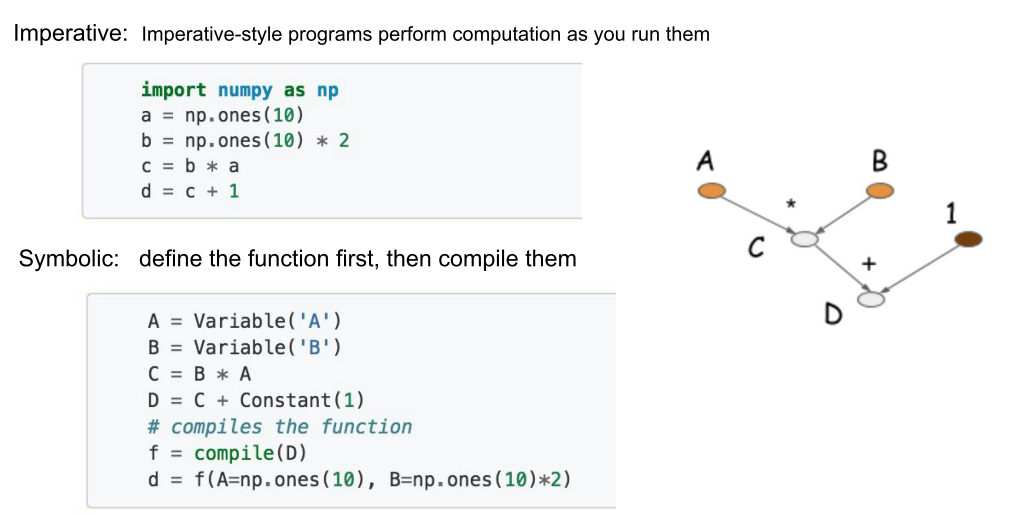
\includegraphics[width=0.9\linewidth,keepaspectratio]{pytorch1}
\end{center}

  {\tiny (Ref: Pytorch Tutorial - Chongruo Wu)}

\end{frame}

%%%%%%%%%%%%%%%%%%%%%%%%%%%%%%%%%%%%%%%%%%%%%%%%%%%
\begin{frame}[fragile] \frametitle{Popular Deep Learning Frameworks}


\begin{center}
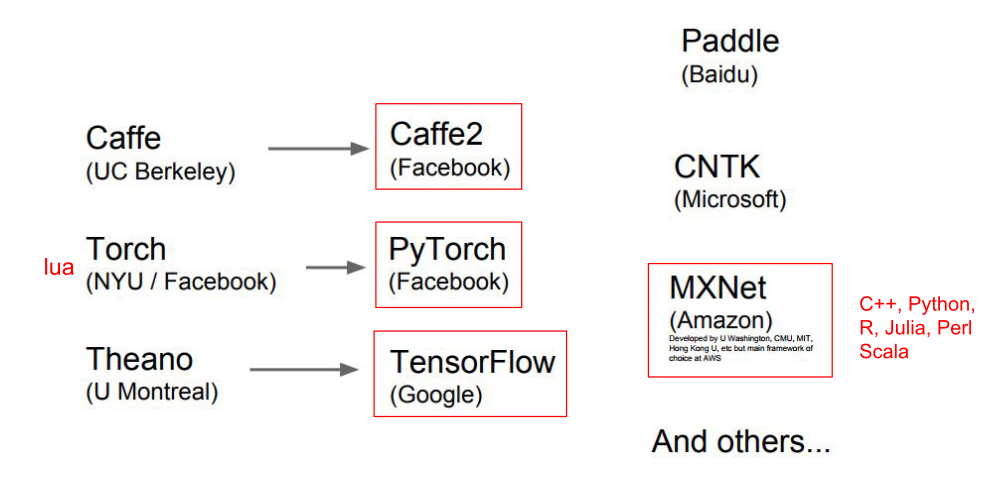
\includegraphics[width=0.9\linewidth,keepaspectratio]{pytorch2}
\end{center}

  {\tiny (Ref: Pytorch Tutorial - Chongruo Wu)}

\end{frame}



%%%%%%%%%%%%%%%%%%%%%%%%%%%%%%%%%%%%%%%%%%%%%%%%%%%
\begin{frame}[fragile] \frametitle{Installation}

Visit https://pytorch.org/get-started/locally/

\begin{center}
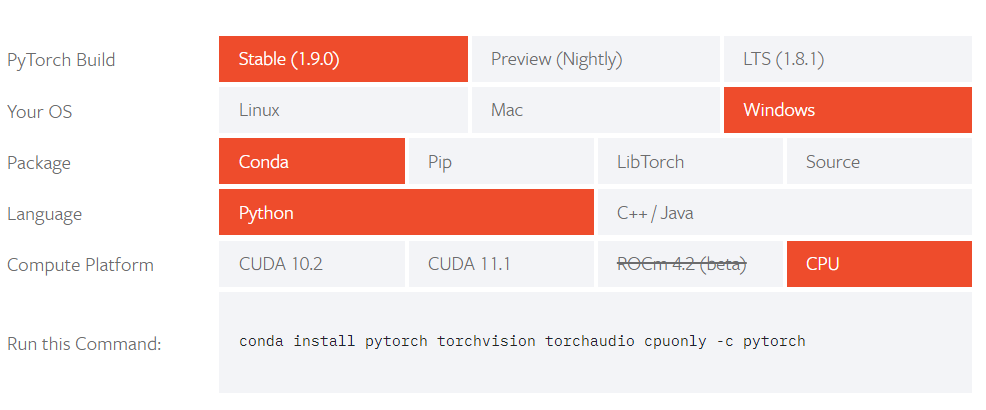
\includegraphics[width=\linewidth,keepaspectratio]{pyt39}%{pyt5}
\end{center}


\end{frame}


%%%%%%%%%%%%%%%%%%%%%%%%%%%%%%%%%%%%%%%%%%%%%%%%%%%
\begin{frame}[fragile] \frametitle{Imp Packages inside PyTorch}
\begin{itemize}
\item  torch: a Tensor library like Numpy, with strong GPU support
\item torch.autograd: an automatic differentiation library 
\item torch.nn: a neural networks library deeply integrated with autograd 
\item torch.optim: an optimization package to be used with torch.nn
\item torch.utils: DataLoader, Trainer and other utility functions for convenience
\end{itemize}
\end{frame}


%%%%%%%%%%%%%%%%%%%%%%%%%%%%%%%%%%%%%%%%%%%%%%%%%%%
\begin{frame}[fragile] \frametitle{Concepts of PyTorch}
\begin{itemize}
\item Data:
\begin{itemize}
\item Tensor
\item Variable (for Gradient)
\end{itemize}
\item Function:
\begin{itemize}
\item   NN Modules
\item   Optimizer
\item   Loss Function
\item   Multi-Processing
\end{itemize}
\end{itemize}
\end{frame}

 % %%%%%%%%%%%%%%%%%%%%%%%%%%%%%%%%%%%%%%%%%%%%%%%%%%%%%%%%%%%%%%%%%%%%%%%%%%%%%%%%%%
\begin{frame}[fragile]
\frametitle{What is a Tensor?}
\begin{itemize}
\item Tensors to encode the inputs and outputs of a model, as well as the model's parameters.
\item Similar to NumPy's ndarrays, except that tensors can run on GPUs or other hardware accelerators. (both actually share same underlying memory, if CPU)

\end{itemize}

 \begin{lstlisting}
import torch
import numpy as np

data = [[1, 2],[3, 4]]
x_data = torch.tensor(data)
x_data_numpy = x_data.numpy()

np_array = np.array(data)
x_np = torch.from_numpy(np_array)

 \end{lstlisting}
 
 
 \end{frame} 
 
 
 % %%%%%%%%%%%%%%%%%%%%%%%%%%%%%%%%%%%%%%%%%%%%%%%%%%%%%%%%%%%%%%%%%%%%%%%%%%%%%%%%%%
\begin{frame}[fragile]
\frametitle{What is a Tensor?}
\begin{itemize}
\item All of deep learning is computations on tensors
\item Array with dimension 0 is a scalar
\item Array with dimension 1 is a vector
\item Array with dimension 2 is a martix
\item Array with dimension 3 or more is a tensor
\item Tensors can be created from Python lists with the torch.tensor() function.
\end{itemize}
 \end{frame} 
 
 % %%%%%%%%%%%%%%%%%%%%%%%%%%%%%%%%%%%%%%%%%%%%%%%%%%%%%%%%%%%%%%%%%%%%%%%%%%%%%%%%%%
\begin{frame}[fragile]
\frametitle{1D Tensor}
1D Vector
 \begin{lstlisting}
 import torch

V_data = [1.,2.,3.]
V = torch.tensor(V_data)
print(V)

>>>tensor([ 1.,  2.,  3.])
 \end{lstlisting}

 \end{frame} 


 
%%%%%%%%%%%%%%%%%%%%%%%%%%%%%%%%%%%%%%%%%%%%%%%%%%%%%%%%%%%%%%%%%%%%%%%%%%%%%%%%%%
\begin{frame}[fragile]
\frametitle{2D Tensor}
Matrix 
 \begin{lstlisting}
M_data = [[1., 2., 3.], [4., 5., 6]]
M = torch.tensor(M_data)
print(M)

>>>tensor([[ 1.,  2.,  3.],
        [ 4.,  5.,  6.]])
 \end{lstlisting}

 \end{frame} 

 
 % %%%%%%%%%%%%%%%%%%%%%%%%%%%%%%%%%%%%%%%%%%%%%%%%%%%%%%%%%%%%%%%%%%%%%%%%%%%%%%%%%%
\begin{frame}[fragile]
\frametitle{3D Tensor}
3D tensor of size 2x2x2.
 \begin{lstlisting}
T_data = [[[1.,2.], [3.,4.]],
          [[5.,6.], [7.,8.]]]
T = torch.tensor(T_data)
print(T)


>>>tensor([[[ 1.,  2.],
         [ 3.,  4.]],

        [[ 5.,  6.],
         [ 7.,  8.]]])
 \end{lstlisting}

 \end{frame} 
 
  % %%%%%%%%%%%%%%%%%%%%%%%%%%%%%%%%%%%%%%%%%%%%%%%%%%%%%%%%%%%%%%%%%%%%%%%%%%%%%%%%%%
\begin{frame}[fragile]
\frametitle{Random, Constant Tensor}

\begin{lstlisting}
shape = (2,3,)
rand_tensor = torch.rand(shape)
ones_tensor = torch.ones(shape)
zeros_tensor = torch.zeros(shape)

print(f"Random Tensor: \n {rand_tensor} \n")
print(f"Ones Tensor: \n {ones_tensor} \n")
print(f"Zeros Tensor: \n {zeros_tensor}")

Random Tensor: 
 tensor([[0.5742, 0.4606, 0.0981],
        [0.3154, 0.0503, 0.0097]]) 

Ones Tensor: 
 tensor([[1., 1., 1.],
        [1., 1., 1.]]) 

Zeros Tensor: 
 tensor([[0., 0., 0.],
        [0., 0., 0.]])
 \end{lstlisting}

 \end{frame} 
 

 % %%%%%%%%%%%%%%%%%%%%%%%%%%%%%%%%%%%%%%%%%%%%%%%%%%%%%%%%%%%%%%%%%%%%%%%%%%%%%%%%%%
\begin{frame}[fragile]
\frametitle{Attributes of Tensor}

\begin{lstlisting}
tensor = torch.rand(3,4)

print(f"Shape of tensor: {tensor.shape}")
print(f"Datatype of tensor: {tensor.dtype}")
print(f"Device tensor is stored on: {tensor.device}")

Shape of tensor: torch.Size([3, 4])
Datatype of tensor: torch.float32
Device tensor is stored on: cpu
 \end{lstlisting}

 \end{frame} 
 
 
 % %%%%%%%%%%%%%%%%%%%%%%%%%%%%%%%%%%%%%%%%%%%%%%%%%%%%%%%%%%%%%%%%%%%%%%%%%%%%%%%%%%
\begin{frame}[fragile]
\frametitle{Indexing}
\begin{itemize}
\item Indexing into the vector gives you a scalar. 
\item Indexing into the matrix gives you a vector. 
\item Indexing into the tensor gives you a matrix!
\end{itemize}

 \begin{lstlisting}
print(V[0])
print(M[0])
print(T[0])

tensor(1.)
tensor([ 1.,  2.,  3.])
tensor([[ 1.,  2.],
        [ 3.,  4.]])
 \end{lstlisting}

 \end{frame} 
 
 
  % %%%%%%%%%%%%%%%%%%%%%%%%%%%%%%%%%%%%%%%%%%%%%%%%%%%%%%%%%%%%%%%%%%%%%%%%%%%%%%%%%%
\begin{frame}[fragile]
\frametitle{Data type}
\begin{itemize}
\item Default datatype in tensor is Float
\item For int tensor, call torch.LongTensor(), etc
\item To create a tensor with random data and the supplied dimensionality with torch.rand()
\end{itemize}

 \end{frame} 
 
%%%%%%%%%%%%%%%%%%%%%%%%%%%%%%%%%%%%%%%%%%%%%%%%%%%%%%%%%%%%%%%%%%%%%%%%%%%%%%%%%%
\begin{frame}[fragile]
\frametitle{Initialization}
 \begin{lstlisting}
x = torch.rand((3, 4, 5))
print(x)

>>>tensor([[[-1.5256, -0.7502, -0.6540, -1.6095, -0.1002],
         [-0.6092, -0.9798, -1.6091, -0.7121,  0.3037],
         [-0.7773, -0.2515, -0.2223,  1.6871,  0.2284],
         [ 0.4676, -0.6970, -1.1608,  0.6995,  0.1991]],

        [[ 0.8657,  0.2444, -0.6629,  0.8073,  1.1017],
         [-0.1759, -2.2456, -1.4465,  0.0612, -0.6177],
         [-0.7981, -0.1316,  1.8793, -0.0721,  0.1578],
         [-0.7735,  0.1991,  0.0457,  0.1530, -0.4757]],

        [[-0.1110,  0.2927, -0.1578, -0.0288,  0.4533],
         [ 1.1422,  0.2486, -1.7754, -0.0255, -1.0233],
         [-0.5962, -1.0055,  0.4285,  1.4761, -1.7869],
         [ 1.6103, -0.7040, -0.1853, -0.9962, -0.8313]]])
 \end{lstlisting}

 \end{frame} 
 
  % %%%%%%%%%%%%%%%%%%%%%%%%%%%%%%%%%%%%%%%%%%%%%%%%%%%%%%%%%%%%%%%%%%%%%%%%%%%%%%%%%%
\begin{frame}[fragile]
\frametitle{Operations on Tensors}
\begin{itemize}
\item 100s of operations available.
\item Each of these operations can be run on the GPU (at typically higher speeds than on a CPU).
\item By default, tensors are created on the CPU. 
\item Need to explicitly move tensors to the GPU using $.to$ method (after checking for GPU availability). 
\item Keep in mind that copying large tensors across devices can be expensive in terms of time and memory!
\end{itemize}

 \begin{lstlisting}
# We move our tensor to the GPU if available
if torch.cuda.is_available():
  tensor = tensor.to('cuda')
 \end{lstlisting}

 \end{frame} 
 
 
 
 %%%%%%%%%%%%%%%%%%%%%%%%%%%%%%%%%%%%%%%%%%%%%%%%%%%%%%%%%%%%%%%%%%%%%%%%%%%%%%%%%%
\begin{frame}[fragile]
\frametitle{Operations}
Operations with Tensors
 \begin{lstlisting}
x = torch.tensor([1.,2.,3.])
y = torch.tensor([4.,5.,6.])
z = x + y
print(z)

>>>tensor([ 5.,  7.,  9.])

 \end{lstlisting}
 
 Operations that store the result into the operand are called in-place. They are denoted by a \lstinline|_| suffix. For example: \lstinline|x.copy_(y), x.t_()|, will change x.
 
  \begin{lstlisting}
tensor.add_(5)
 \end{lstlisting}
 
 Note:  In-place operations save some memory, but can be problematic when computing derivatives because of an immediate loss of history. Hence, their use is discouraged.
 \end{frame} 
 
 %%%%%%%%%%%%%%%%%%%%%%%%%%%%%%%%%%%%%%%%%%%%%%%%%%%%%%%%%%%%%%%%%%%%%%%%%%%%%%%%%%
\begin{frame}[fragile]
\frametitle{Operations}
Multiplication

\begin{lstlisting}
# This computes the matrix multiplication between two tensors. y1, y2, y3 will have the same value
y1 = tensor @ tensor.T
y2 = tensor.matmul(tensor.T)

y3 = torch.rand_like(tensor)
torch.matmul(tensor, tensor.T, out=y3)


# This computes the element-wise product. z1, z2, z3 will have the same value
z1 = tensor * tensor
z2 = tensor.mul(tensor)

z3 = torch.rand_like(tensor)
torch.mul(tensor, tensor, out=z3)
 \end{lstlisting}
Many more mathematical operations are available.
 \end{frame} 
 
 
%%%%%%%%%%%%%%%%%%%%%%%%%%%%%%%%%%%%%%%%%%%%%%%%%%%%%%%%%%%%%%%%%%%%%%%%%%%%%%%%%%
\begin{frame}[fragile]
\frametitle{Concatenation}
Concatenation
 \begin{lstlisting}
# By default, it concatenates along the first axis (concatenates rows)
x_1 = torch.randn(2, 5)
y_1 = torch.randn(3, 5)
z_1 =torch.cat([x_1, y_1])
print(z_1)

# Concatenate columns:
x_2 = torch.randn(2, 3)
y_2 = torch.randn(2, 5)
z_2 = torch.cat([x_2, y_2], 1) # second arg specifies which axis to concat along
print(z_2)

# If your tensors are not compatible, torch will complain.  Uncomment to see the error
# torch.cat([x_1, x_2])
 \end{lstlisting}
 \end{frame} 
 
 %%%%%%%%%%%%%%%%%%%%%%%%%%%%%%%%%%%%%%%%%%%%%%%%%%%%%%%%%%%%%%%%%%%%%%%%%%%%%%%%%%
\begin{frame}[fragile]
\frametitle{Reshaping}
Reshaping Tensors with view() method.
 \begin{lstlisting}
x = torch.randn(2,3,4)
print(x)
print(x.view(2,12)) # Reshape to 2 rows, 12 columns
print(x.view(2, -1)) # Same as above. 
 \end{lstlisting}
  If one of the dimensions is -1, its size can be inferred
 \end{frame} 
 
%%%%%%%%%%%%%%%%%%%%%%%%%%%%%%%%%%%%%%%%%%%%%%%%%%%%%%%%%%%%%%%%%%%%%%%%%%%%%%%%%%
\begin{frame}[fragile]
\frametitle{Computation Graphs}

\begin{itemize}
\item It is a specification of how your data is combined to give you the output. 
\item Since the graph totally specifies what parameters were involved with which operations, it contains enough information to compute derivatives.
\end{itemize}
 \end{frame} 
 
 
 %%%%%%%%%%%%%%%%%%%%%%%%%%%%%%%%%%%%%%%%%%%%%%%%%%%%%%%%%%%%%%%%%%%%%%%%%%%%%%%%%%
\begin{frame}[fragile]
\frametitle{Variables and Tensors}
\begin{itemize}
\item What does torch.tensor object has stored? : data and the shape, and maybe a few other things
\item But when we added two tensors together, we got an output tensor. 
\item All this output tensor knows is its data and shape. 
\item It has no idea that it was the sum of two other tensors (it could have been read in from a file, it could be the result of some other operation, etc.)
\item The Variable class keeps track of how it was created. 
\end{itemize}
Latest News: Variables and Tensors have merged!!!
 \end{frame} 
 
 
%%%%%%%%%%%%%%%%%%%%%%%%%%%%%%%%%%%%%%%%%%%%%%%%%%%%%%%%%%%%%%%%%%%%%%%%%%%%%%%%%%
\begin{frame}[fragile]
\frametitle{PyTorch 0.4.0 release notes}
\begin{itemize}
\item Tensors and Variables have merged
\item torch.autograd.Variable and torch.tensor are now the same class. 
\item More precisely, torch.tensor is capable of tracking history and behaves like the old Variable; Variable wrapping continues to work as before but returns an object of type torch.tensor. \item No need the Variable wrapper everywhere in your code anymore.
\end{itemize}
 \begin{lstlisting}
>>> x = torch.DoubleTensor([1, 1, 1])
>>> print(type(x)) # was torch.DoubleTensor
<class 'torch.autograd.variable.Variable'>
>>> print(x.type())  # OK: 'torch.DoubleTensor'
'torch.DoubleTensor'
>>> print(isinstance(x, torch.DoubleTensor))  # OK: True
True
 \end{lstlisting}
 \end{frame} 
 
    %%%%%%%%%%%%%%%%%%%%%%%%%%%%%%%%%%%%%%%%%%%%%%%%%%%%%%%%%%%%%%%%%%%%%%%%%%%%%%%%%%
\begin{frame}[fragile]
\frametitle{PyTorch 0.4.0 release notes}

\begin{itemize}
\item When does autograd start tracking history now?
\item requires\_grad, the central flag for autograd, is now an attribute on Tensors.
\end{itemize}
 \begin{lstlisting}
>>> x = torch.ones(1)  # create a tensor with requires_grad=False (default)
>>> x.requires_grad
False
>>> y = torch.ones(1)  # another tensor with requires_grad=False
>>> z = x + y
>>> # both inputs have requires_grad=False. so does the output
>>> z.requires_grad
False
>>> # then autograd won't track this computation. let's verify!
>>> z.backward()
RuntimeError: element 0 of tensors does not require grad and does not have a grad_fn
 \end{lstlisting}
 \end{frame} 
 
     %%%%%%%%%%%%%%%%%%%%%%%%%%%%%%%%%%%%%%%%%%%%%%%%%%%%%%%%%%%%%%%%%%%%%%%%%%%%%%%%%%
\begin{frame}[fragile]
\frametitle{PyTorch 0.4.0 release notes}

 \begin{lstlisting}
>>>
>>> # now create a tensor with requires_grad=True
>>> w = torch.ones(1, requires_grad=True)
>>> w.requires_grad
True
>>> # add to the previous result that has require_grad=False
>>> total = w + z
>>> # the total sum now requires grad!
>>> total.requires_grad
True
>>> # autograd can compute the gradients as well
>>> total.backward()
>>> w.grad
tensor([ 1.])
>>> # and no computation is wasted to compute gradients for x, y and z, which don't require grad
>>> z.grad == x.grad == y.grad == None
True
 \end{lstlisting}
 \end{frame} 
 
     %%%%%%%%%%%%%%%%%%%%%%%%%%%%%%%%%%%%%%%%%%%%%%%%%%%%%%%%%%%%%%%%%%%%%%%%%%%%%%%%%%
\begin{frame}[fragile]
\frametitle{PyTorch 0.4.0 release notes}

\begin{itemize}
\item What about .data?
\item .data was the primary way to get the underlying Tensor from a Variable. 
\item After this merge, calling y = x.data still has similar semantics.
\item So y will be a Tensor that shares the same data with x, is unrelated with the computation history of x, and has requires\_grad=False.
\end{itemize}

From now onwards, even if Variables and Tensors are mentioned disticnlty, from 0.4.0, they are just the Tensors with grad\_fn available.
\end{frame} 
 
 
  
  %%%%%%%%%%%%%%%%%%%%%%%%%%%%%%%%%%%%%%%%%%%%%%%%%%%%%%%%%%%%%%%%%%%%%%%%%%%%%%%%%%
\begin{frame}[fragile]
\frametitle{Tensor/Variables operations}

 \begin{lstlisting}
x = torch.tensor([1.,2.,3.])
y = torch.tensor([4.,5.,6.])
x.requires_grad = True
y.requires_grad = True
z = x + y
print(z.data)
>>>tensor([ 5.,  7.,  9.])
print(z.grad_fn)
>>><AddBackward1 object at 0x000000000A9C94A8>
s = z.sum()
print(s.data)
>>>tensor(21.)
print(s.grad_fn)
>>><SumBackward0 object at 0x000000000A9C94E0>
 \end{lstlisting}
So now, what is the derivative of this sum with respect to the first component of x? 
 \end{frame} 
 
%%%%%%%%%%%%%%%%%%%%%%%%%%%%%%%%%%%%%%%%%%%%%%%%%%%%%%%%%%%%%%%%%%%%%%%%%%%%%%%%%%
\begin{frame}[fragile]
\frametitle{Derivative}
\begin{itemize}
\item Need $\frac{\partial s}{\partial x_0}$
\item s knows that it was created as a sum of the tensor z. 
\item z knows that it was the sum x + y. 
\item So, $s = \overbrace{x_0 + y_0}^\text{$z_0$} + \overbrace{x_1 + y_1}^\text{$z_1$} + \overbrace{x_2 + y_2}^\text{$z_2$}$
\item Enough information to determine that the derivative : Pytorch knows how to compute their gradients of sum() and + operations, and run the back propagation algorithm. 
\end{itemize}


\end{frame} 
 
 %%%%%%%%%%%%%%%%%%%%%%%%%%%%%%%%%%%%%%%%%%%%%%%%%%%%%%%%%%%%%%%%%%%%%%%%%%%%%%%%%%
\begin{frame}[fragile]
\frametitle{Back Propagation}

 \begin{lstlisting}
s.backward() # calling .backward() on any variable will run backprop, starting from it.
print(x.grad)

>>>tensor([ 1.,  1.,  1.])
 \end{lstlisting}

\end{frame} 
 
 
  %%%%%%%%%%%%%%%%%%%%%%%%%%%%%%%%%%%%%%%%%%%%%%%%%%%%%%%%%%%%%%%%%%%%%%%%%%%%%%%%%%
\begin{frame}[fragile]
\frametitle{Variable Gradient}
Note:
 \begin{lstlisting}
x = torch.randn((2,2))
y = torch.randn((2,2))
x.requires_grad = True
y.requires_grad = True
z = x + y 
print(z.grad_fn)
>>><AddBackward1 object at 0x000000000A9D2358>

var_z_data = z.data # Get the wrapped Tensor object out of var_z...
new_var_z = torch.tensor( var_z_data ) # Re-wrap the tensor in a new variable

# does new_var_z have info to backprop to x and y? NO!
print(new_var_z.grad_fn)
>>>None
# And how could it?  We copied the tensor values out of z (that is what z.data is).  This tensor doesn't know anything about how it was computed.   If var_z_data doesn't know how it was computed, theres no way new_var_z will.
\end{lstlisting}

\end{frame} 
 

%%%%%%%%%%%%%%%%%%%%%%%%%%%%%%%%%%%%%%%%%%%%%%%%%%%
\begin{frame}[fragile] \frametitle{Autograd: automatic gradient}
\begin{itemize}
\item Provides automatic differentiation for all operations on Tensors
\item It is a define-by-run framework, which means that your backprop is defined by how your code is run, and that every single iteration can be different.
\end{itemize}
\end{frame}

%%%%%%%%%%%%%%%%%%%%%%%%%%%%%%%%%%%%%%%%%%%%%%%%%%%
\begin{frame}[fragile] \frametitle{Automatic differentiation}

\begin{itemize}
\item In $backpropogation$ parameters (model weights) are adjusted according to the gradient of the loss function with respect to the given parameter.
\item To compute those gradients, PyTorch has a built-in differentiation engine called \lstinline|torch.autograd|. 
\item It supports automatic computation of gradient for any computational graph.
\item Consider the simplest one-layer neural network, with input x, parameters w and b, and some loss function.
\end{itemize}

\begin{lstlisting}
import torch

x = torch.ones(5)  # input tensor
y = torch.zeros(3)  # expected output
w = torch.randn(5, 3, requires_grad=True)
b = torch.randn(3, requires_grad=True)
z = torch.matmul(x, w)+b
loss = torch.nn.functional.binary_cross_entropy_with_logits(z, y)
\end{lstlisting}

\tiny{(Ref: Microsoft - Intro to Machine Learning using Pytorch)}
\end{frame}

%%%%%%%%%%%%%%%%%%%%%%%%%%%%%%%%%%%%%%%%%%%%%%%%%%%
\begin{frame}[fragile] \frametitle{Tensors, Functions and Computational graph}

\begin{center}
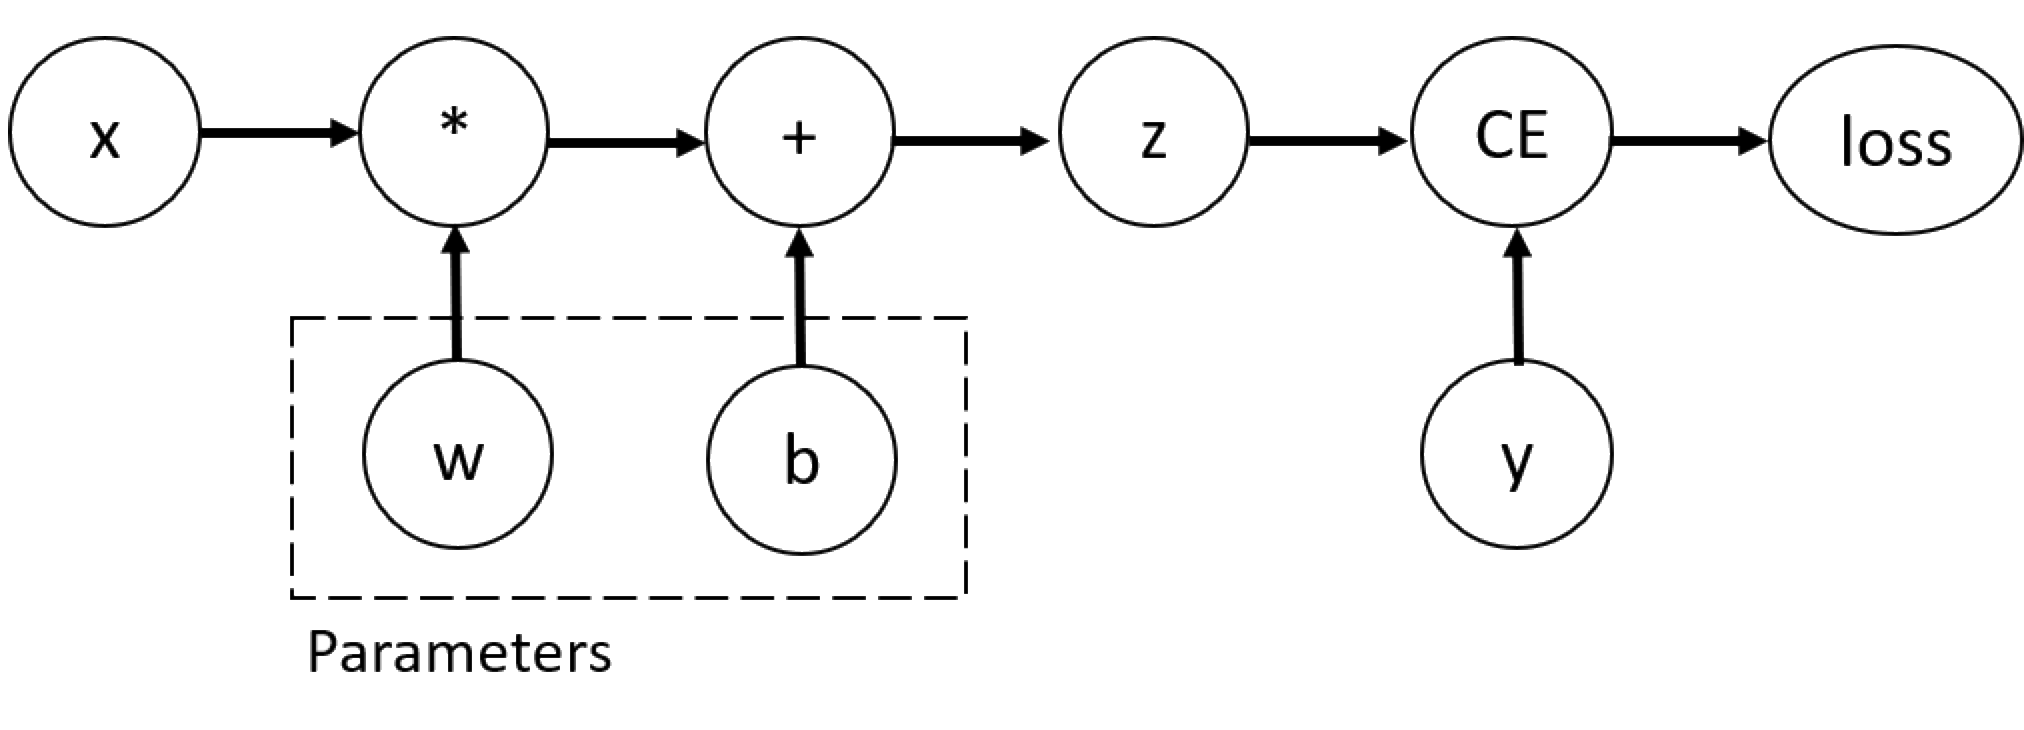
\includegraphics[width=\linewidth,keepaspectratio]{pyt40}
\end{center}

\begin{itemize}
\item In this network, w and b are parameters, which need to be optimized. 
\item Need to be able to compute the gradients of loss function with respect to those variables. 
\item Set the \lstinline|requires_grad| property of those tensors. Note: You can set the value of \lstinline|requires_grad| when creating a tensor, or later by using \lstinline|x.requires_grad_(True)| method.
\end{itemize}


\tiny{(Ref: Microsoft - Intro to Machine Learning using Pytorch)}
\end{frame}

%%%%%%%%%%%%%%%%%%%%%%%%%%%%%%%%%%%%%%%%%%%%%%%%%%%
\begin{frame}[fragile] \frametitle{Tensors, Functions and Computational graph}

\begin{itemize}
\item A function that we apply to tensors to construct computational graph is in fact an object of class Function. 
\item This object knows how to compute the function in the forward direction, and also how to compute its derivative during the backward propagation step. 
\item A reference to the backward propagation function is stored in \lstinline|grad_fn| property of a tensor.
\end{itemize}

\begin{lstlisting}
print('Gradient function for z =',z.grad_fn)
print('Gradient function for loss =', loss.grad_fn)

>>>Gradient function for z = <AddBackward0 object at 0x7fcaa4928110>
Gradient function for loss = <BinaryCrossEntropyWithLogitsBackward object at 0x7fcaa4928250>
\end{lstlisting}

\tiny{(Ref: Microsoft - Intro to Machine Learning using Pytorch)}
\end{frame}

%%%%%%%%%%%%%%%%%%%%%%%%%%%%%%%%%%%%%%%%%%%%%%%%%%%
\begin{frame}[fragile] \frametitle{Computing gradients}

\begin{itemize}
\item To optimize weights of parameters in the neural network, we need to compute the derivatives of our loss function with respect to parameters, namely, we need  $\frac{\partial loss}{\partial w}$ and
$\frac{\partial loss}{\partial b}$   under some fixed values of x and y. 
\item To compute those derivatives, we call \lstinline|loss.backward()|, and then retrieve the values from \lstinline|w.grad| and \lstinline|b.grad|:
\end{itemize}

\begin{lstlisting}
loss.backward()
print(w.grad)
print(b.grad)

>>>tensor([[0.2739, 0.0490, 0.3279],
        [0.2739, 0.0490, 0.3279],
        [0.2739, 0.0490, 0.3279],
        [0.2739, 0.0490, 0.3279],
        [0.2739, 0.0490, 0.3279]])
tensor([0.2739, 0.0490, 0.3279])
\end{lstlisting}

\tiny{(Ref: Microsoft - Intro to Machine Learning using Pytorch)}
\end{frame}

%%%%%%%%%%%%%%%%%%%%%%%%%%%%%%%%%%%%%%%%%%%%%%%%%%%
\begin{frame}[fragile] \frametitle{Computing gradients}

Note:
\begin{itemize}
\item We can only obtain the grad properties for the leaf nodes of the computational graph, which have \lstinline|requires_grad| property set to True. 
\item For all other nodes in our graph, gradients will not be available. 
\item In addition, we can only perform gradient calculations using backward once on a given graph, for performance reasons. 
\item If we need to do several backward calls on the same graph, we need to pass \lstinline|retain_graph=True| to the backward call.
\item By default, all tensors with \lstinline|requires_grad=True| are tracking their computational history and support gradient computation. 
\item However, if we only want to do forward computations through the network. We can stop tracking computations by surrounding our computation code with \lstinline|torch.no_grad()| block.
\item Disabling can also be used to mark some parameters in your neural network at frozen parameters, say, for pre-trained networks.
\end{itemize}

\begin{lstlisting}
z = torch.matmul(x, w)+b
print(z.requires_grad)

with torch.no_grad():
    z = torch.matmul(x, w)+b
print(z.requires_grad)

>>>True
False
\end{lstlisting}

\tiny{(Ref: Microsoft - Intro to Machine Learning using Pytorch)}
\end{frame}


%%%%%%%%%%%%%%%%%%%%%%%%%%%%%%%%%%%%%%%%%%%%%%%%%%%
\begin{frame}[fragile] \frametitle{Computional Graphs}


\begin{itemize}
\item Conceptually, autograd keeps a record of data (tensors) and all executed operations (along with the resulting new tensors) in a directed acyclic graph (DAG) consisting of Function objects. 
\item In this DAG, leaves are the input tensors, roots are the output tensors. 
\item By tracing this graph from roots to leaves, you can automatically compute the gradients using the chain rule.
\item In a forward pass, autograd does two things simultaneously:
	\begin{itemize}
	\item run the requested operation to compute a resulting tensor
	\item maintain the operation’s gradient function in the DAG.
	\end{itemize}
\item The backward pass kicks off when .backward() is called on the DAG root. autograd then:
	\begin{itemize}
	\item computes the gradients from each \lstinline|.grad_fn|,
	\item accumulates them in the respective tensor’s \lstinline|.grad| attribute
	\item using the chain rule, propagates all the way to the leaf tensors.
	\end{itemize}

\end{itemize}


\tiny{(Ref: Microsoft - Intro to Machine Learning using Pytorch)}
\end{frame}

%%%%%%%%%%%%%%%%%%%%%%%%%%%%%%%%%%%%%%%%%%%%%%%%%%%
\begin{frame}[fragile] \frametitle{Computional Graphs}
DAGs are dynamic in PyTorch

\begin{itemize}
\item The graph is recreated from scratch; after each \lstinline|.backward()| call, autograd starts populating a new graph. 
\item This is exactly what allows you to use control flow statements in your model; you can change the shape, size and operations at every iteration if needed.
\end{itemize}


\tiny{(Ref: Microsoft - Intro to Machine Learning using Pytorch)}
\end{frame}

%%%%%%%%%%%%%%%%%%%%%%%%%%%%%%%%%%%%%%%%%%%%%%%%%%%
\begin{frame}[fragile] \frametitle{Computional Graphs}
Odd cases
\begin{itemize}
\item In case of a scalar loss function, and we need to compute the gradient with respect to some parameters. 
\item However, there are cases when the output function is an arbitrary tensor. 
\item In this case, PyTorch allows you to compute so-called Jacobian product, and not the actual gradient.
\item For a vector function $\vec{y}=f(\vec{x})$, where
$\vec{x}=\langle x_1,\dots,x_n\rangle$ and
$\vec{y}=\langle y_1,\dots,y_m\rangle$, a gradient of
$\vec{y}$ with respect to $\vec{x}$ is given by \lstinline|Jacobian matrix|

% \begin{align}
% \begin{align}J=\left(\begin{array}{ccc}
      % \frac{\partial y_{1}}{\partial x_{1}} & \cdots & \frac{\partial y_{1}}{\partial x_{n}}\\
      % \vdots & \ddots & \vdots\\
      % \frac{\partial y_{m}}{\partial x_{1}} & \cdots & \frac{\partial y_{m}}{\partial x_{n}}
      % \end{array}\right)
% \end{align}
% \end{align}

\item Instead of computing the Jacobian matrix itself, PyTorch allows you to
compute **Jacobian Product** $v^T\cdot J$ for a given input vector
$v=(v_1 \dots v_m)$. This is achieved by calling `backward` with
$v$ as an argument. The size of $v$ should be the same as
the size of the original tensor, with respect to which we want to
compute the product
\end{itemize}


\tiny{(Ref: Microsoft - Intro to Machine Learning using Pytorch)}
\end{frame}


%%%%%%%%%%%%%%%%%%%%%%%%%%%%%%%%%%%%%%%%%%%%%%%%%%%
\begin{frame}[fragile] \frametitle{Computional Graphs}

\begin{lstlisting}
inp = torch.eye(5, requires_grad=True)
out = (inp+1).pow(2)
out.backward(torch.ones_like(inp), retain_graph=True)
print("First call\n", inp.grad)
out.backward(torch.ones_like(inp), retain_graph=True)
print("\nSecond call\n", inp.grad)
inp.grad.zero_()
out.backward(torch.ones_like(inp), retain_graph=True)
print("\nCall after zeroing gradients\n", inp.grad)

\end{lstlisting}

\begin{itemize}
\item Notice that when we call backward for the second time with the same argument, the value of the gradient is different. 
\item This happens because PyTorch accumulates the gradients, i.e. the value of computed gradients is added to the grad property of all leaf nodes of computational graph. 
\item If you want to compute the proper gradients, you need to zero out the grad property before. 
\item \lstinline|backward()| is equivalent to calling \lstinline|backward(torch.tensor(1.0))|, which is a useful way to compute the gradients in case of a scalar-valued function, such as loss during neural network training.
\end{itemize}


\tiny{(Ref: Microsoft - Intro to Machine Learning using Pytorch)}
\end{frame}

% %%%%%%%%%%%%%%%%%%%%%%%%%%%%%%%%%%%%%%%%%%%%%%%%%%%
% \begin{frame}[fragile] \frametitle{Function}
% \begin{itemize}
% \item Implements forward and backward definitions of an autograd operation. 
% \item Every Variable operation, creates at least a single Function node, that connects to functions that created a Variable and encodes its history.
% \item Variable and Function are interconnected and build up an acyclic graph, that encodes a complete history of computation.
% \item Each variable has a .grad\_fn attribute that references a Function that has created the Variable (except for Variables created by the user - their grad\_fn is None).
% \end{itemize}
% \end{frame}

%%%%%%%%%%%%%%%%%%%%%%%%%%%%%%%%%%%%%%%%%%%%%%%%%%%%%%%%%%%%%%%%%%%%%%%%%%%%%%%%%%
\begin{frame}[fragile]
\frametitle{Activation Functions}

\begin{itemize}
\item Neural network consists of composing linearities with non-linearities, a long chains of affine compositions.
\item Non-linearities like $\tanh(x), \sigma(x), \text{ReLU}(x)$ are the most common.
\item Why these functions? I can think of plenty of other non-linearities.
\end{itemize}
\end{frame} 

%%%%%%%%%%%%%%%%%%%%%%%%%%%%%%%%%%%%%%%%%%%%%%%%%%%%%%%%%%%%%%%%%%%%%%%%%%%%%%%%%%
\begin{frame}[fragile]
\frametitle{Activation}

\begin{itemize}
\item The reason for this is that they have gradients that are easy to compute, and computing gradients is essential for learning. For example $ \frac{d\sigma}{dx} = \sigma(x)(1 - \sigma(x)) $
\item $ \sigma(x)$ less popular because the gradient vanishes very quickly as the absolute value of the argument grows. Small gradients means it is hard to learn. Most use tanh or ReLU.
\end{itemize}
 \begin{lstlisting}
data = torch.randn(2,2,requires_grad=True)
print(data)
import torch.nn.functional as F
print(F.relu(data))
>>>tensor([[ 1.6169, -0.9026],
        [ 0.1737,  0.0772]])
tensor([[ 1.6169,  0.0000],
        [ 0.1737,  0.0772]])
 \end{lstlisting}
 Note, all negatives are made 0 and positives kept as they are.
\end{frame} 

%%%%%%%%%%%%%%%%%%%%%%%%%%%%%%%%%%%%%%%%%%%%%%%%%%%%%%%%%%%%%%%%%%%%%%%%%%%%%%%%%%
\begin{frame}[fragile]
\frametitle{Softmax and Probabilities}

\begin{itemize}
\item The function $\text{Softmax}(x)$ is also just a non-linearity, but it is special in that it usually is the last operation done in a network. 
\item This is because it takes in a vector of real numbers and returns a probability distribution.
\end{itemize}
 \begin{lstlisting}
data = torch.randn(5,requires_grad=True)
print(data)
print(F.softmax(data,0))
print(F.softmax(data,0).sum())

>>>tensor([ 0.1896, -0.2204,  0.1491,  0.0100, -0.1243])
tensor([ 0.2387,  0.1584,  0.2292,  0.1994,  0.1744])
tensor(1.)
 \end{lstlisting}
It should be clear that the output is a probability distribution: each element is non-negative and the sum over all components is 1.
\end{frame} 

%%%%%%%%%%%%%%%%%%%%%%%%%%%%%%%%%%%%%%%%%%%%%%%%%%%%%%%%%%%%%%%%%%%%%%%%%%%%%%%%%%
\begin{frame}[fragile]
\frametitle{Objective or Loss or Cost function}

\begin{itemize}
\item Neural network is being trained to minimize it.
\item The parameters of the model are then updated by taking the derivative of the loss function. 
\item An example loss function is the negative log likelihood loss, which is a very common objective for multi-class classification.
\item We can compute gradients with respect to all of the parameters used to compute it! Then we can perform standard gradient updates.
\item Let $\theta$ be our parameters,  $L(\theta)$ the loss function, and $\eta$ a positive learning rate. Then:

$$ \theta^{(t+1)} = \theta^{(t)} - \eta \nabla_\theta L(\theta) $$
\end{itemize}

\end{frame} 

%%%%%%%%%%%%%%%%%%%%%%%%%%%%%%%%%%%%%%%%%%%%%%%%%%%%%%%%%%%%%%%%%%%%%%%%%%%%%%%%%%
\begin{frame}[fragile]
\frametitle{Optimization}

\begin{itemize}
\item Training a model is an iterative process; in each iteration (called an epoch) the model makes a guess about the output, calculates the error in its guess (loss), collects the derivatives of the error with respect to its parameters (as we saw in the module), and optimizes these parameters using gradient descent.
\item Many optimization methods do something more than just this vanilla gradient update.
\item Many attempt to vary the learning rate based on what is happening at train time. 
\item Torch provies many in the torch.optim package, and they are all completely transparent. 
\item Using the simplest gradient update is the same as the more complicated algorithms. 
\item Trying different algorithms and different parameters 
\item Other choices: Adam or RMSProp will boost performance noticably.
\end{itemize}

\end{frame} 

%%%%%%%%%%%%%%%%%%%%%%%%%%%%%%%%%%%%%%%%%%%%%%%%%%%
\begin{frame}[fragile] \frametitle{Setting hyperparameters}

Hyperparameters are adjustable parameters that let you control the model optimization process. Example:

\begin{itemize}
\item Number of Epochs: the number times to iterate over the dataset
\item Batch Size: the number of data samples seen by the model in each epoch
\item Learning Rate : how much to update models parameters at each batch/epoch. Smaller values yield slow learning speed, while large values may result in unpredictable behavior during training.
\end{itemize}


\begin{lstlisting}
learning_rate = 1e-3
batch_size = 64
epochs = 5
\end{lstlisting}

Each epoch consists of two main parts:

\begin{itemize}
\item The Train Loop: iterate over the training dataset and try to converge to optimal parameters.
\item The Validation/Test Loop: iterate over the test dataset to check if model performance is improving.
\end{itemize}

\tiny{(Ref: Microsoft - Intro to Machine Learning using Pytorch)}
\end{frame}


%%%%%%%%%%%%%%%%%%%%%%%%%%%%%%%%%%%%%%%%%%%%%%%%%%%
\begin{frame}[fragile] \frametitle{Loss}


\begin{itemize}
\item Loss function measures the degree of dissimilarity of obtained result to the target value, and it is the loss function that we want to minimize during training. \item To calculate the loss we make a prediction using the inputs of our given data sample and compare it against the true data label value.
\item Common loss functions include \lstinline|nn.MSELoss| (Mean Square Error) for regression tasks, and \lstinline|nn.NLLLoss| (Negative Log Likelihood) for classification. 
\item \lstinline|nn.CrossEntropyLoss| combines \lstinline|nn.LogSoftmax| and \lstinline|nn.NLLLoss|.
\end{itemize}


\begin{lstlisting}
# Initialize the loss function
loss_fn = nn.CrossEntropyLoss()
\end{lstlisting}

\tiny{(Ref: Microsoft - Intro to Machine Learning using Pytorch)}
\end{frame}

%%%%%%%%%%%%%%%%%%%%%%%%%%%%%%%%%%%%%%%%%%%%%%%%%%%
\begin{frame}[fragile] \frametitle{Optimization pass}


\begin{itemize}
\item Optimization is the process of adjusting model parameters to reduce model error in each training step. 
\item Optimization algorithms define how this process is performed (in this example we use Stochastic Gradient Descent). 
\item All optimization logic is encapsulated in the optimizer object. Here, we use the SGD optimizer; additionally, there are many different optimizers available in PyTorch such as ADAM and RMSProp, that work better for different kinds of models and data.
\item We initialize the optimizer by registering the model's parameters that need to be trained, and passing in the learning rate hyperparameter.
\end{itemize}


\begin{lstlisting}
optimizer = torch.optim.SGD(model.parameters(), lr=learning_rate)
\end{lstlisting}

\tiny{(Ref: Microsoft - Intro to Machine Learning using Pytorch)}
\end{frame}

%%%%%%%%%%%%%%%%%%%%%%%%%%%%%%%%%%%%%%%%%%%%%%%%%%%
\begin{frame}[fragile] \frametitle{Optimization Pass}

Inside the training loop, optimization happens in three steps:

\begin{itemize}
\item Call \lstinline|optimizer.zero_grad()| to reset the gradients of model parameters. Gradients by default add up; to prevent double-counting, we explicitly zero them at each iteration.
\item Back-propagate the prediction loss with a call to \lstinline|loss.backwards()|. PyTorch deposits the gradients of the loss w.r.t. each parameter.
\item Once we have our gradients, we call \lstinline|optimizer.step()| to adjust the parameters by the gradients collected in the backward pass.
\item We initialize the loss function and optimizer, and pass it to \lstinline|train_loop| and \lstinline|test_loop|.
\end{itemize}


\tiny{(Ref: Microsoft - Intro to Machine Learning using Pytorch)}
\end{frame}

%%%%%%%%%%%%%%%%%%%%%%%%%%%%%%%%%%%%%%%%%%%%%%%%%%%
\begin{frame}[fragile] \frametitle{Training Loop}


\begin{lstlisting}
def train_loop(dataloader, model, loss_fn, optimizer):
    size = len(dataloader.dataset)
    for batch, (X, y) in enumerate(dataloader):        
        # Compute prediction and loss
        pred = model(X)
        loss = loss_fn(pred, y)
        
        # Backpropagation
        optimizer.zero_grad()
        loss.backward()
        optimizer.step()

        if batch % 100 == 0:
            loss, current = loss.item(), batch * len(X)
            print(f"loss: {loss:>7f}  [{current:>5d}/{size:>5d}]")
\end{lstlisting}

\tiny{(Ref: Microsoft - Intro to Machine Learning using Pytorch)}
\end{frame}




%%%%%%%%%%%%%%%%%%%%%%%%%%%%%%%%%%%%%%%%%%%%%%%%%%%
\begin{frame}[fragile] \frametitle{Testing Loop}


\begin{lstlisting}
def test_loop(dataloader, model, loss_fn):
    size = len(dataloader.dataset)
    test_loss, correct = 0, 0

    with torch.no_grad():
        for X, y in dataloader:
            pred = model(X)
            test_loss += loss_fn(pred, y).item()
            correct += (pred.argmax(1) == y).type(torch.float).sum().item()
            
    test_loss /= size
    correct /= size
    print(f"Test Error: \n Accuracy: {(100*correct):>0.1f}%, Avg loss: {test_loss:>8f} \n")
\end{lstlisting}

\tiny{(Ref: Microsoft - Intro to Machine Learning using Pytorch)}
\end{frame}


%%%%%%%%%%%%%%%%%%%%%%%%%%%%%%%%%%%%%%%%%%%%%%%%%%%
\begin{frame}[fragile] \frametitle{Iterations}


\begin{lstlisting}
loss_fn = nn.CrossEntropyLoss()
optimizer = torch.optim.SGD(model.parameters(), lr=learning_rate)

epochs = 10
for t in range(epochs):
    print(f"Epoch {t+1}\n-------------------------------")
    train_loop(train_dataloader, model, loss_fn, optimizer)
    test_loop(test_dataloader, model, loss_fn)
print("Done!")
\end{lstlisting}

\tiny{(Ref: Microsoft - Intro to Machine Learning using Pytorch)}
\end{frame}



%%%%%%%%%%%%%%%%%%%%%%%%%%%%%%%%%%%%%%%%%%%%%%%%%%%
\begin{frame}[fragile] \frametitle{Save and load the model}

\lstinline|torch.save| persists \lstinline|state_dict| which is an internal state dictionary storing the learned parameters.

\begin{lstlisting}
model = models.vgg16(pretrained=True)
torch.save(model.state_dict(), 'data/model_weights.pth')
\end{lstlisting}

\lstinline|load_state_dict()| load the parameters 

\begin{lstlisting}
model = models.vgg16() # we do not specify pretrained=True, i.e. do not load default weights
model.load_state_dict(torch.load('data/model_weights.pth'))
model.eval()
\end{lstlisting}

Note: Be sure to call model.eval() method before inferencing to set the dropout and batch normalization layers to evaluation mode. Failing to do this will yield inconsistent inference results.

\tiny{(Ref: Microsoft - Intro to Machine Learning using Pytorch)}
\end{frame}


%%%%%%%%%%%%%%%%%%%%%%%%%%%%%%%%%%%%%%%%%%%%%%%%%%%
\begin{frame}[fragile] \frametitle{Save and load the model}

If we want to store the architecture also, along with weights then pass the whole model to \lstinline|torch.save|

\begin{lstlisting}
torch.save(model, 'data/vgg_model.pth')
\end{lstlisting}

We can then load the model like this:

\begin{lstlisting}
model = torch.load('data/vgg_model.pth')
\end{lstlisting}

Note: This approach uses Python pickle module when serializing the model, thus it relies on the actual class definition to be available when loading the model.

\tiny{(Ref: Microsoft - Intro to Machine Learning using Pytorch)}
\end{frame}

%%%%%%%%%%%%%%%%%%%%%%%%%%%%%%%%%%%%%%%%%%%%%%%%%%%
\begin{frame}[fragile] \frametitle{ONNX}

\begin{itemize}
\item PyTorch also has native ONNX export support. 
\item Given the dynamic nature of the PyTorch execution graph, however, the export process must traverse the execution graph to produce a persisted ONNX model. 
\item For this reason, a test variable of the appropriate size should be passed in to the export routine (in our case, we will create a dummy zero tensor of the correct size):
\end{itemize}


\begin{lstlisting}
input_image = torch.zeros((1,3,224,224))
onnx.export(model, input_image, 'data/model.onnx')
\end{lstlisting}

There are a lot of things you can do with ONNX model, including running inference on different platforms and in different programming languages. 

\tiny{(Ref: Microsoft - Intro to Machine Learning using Pytorch)}
\end{frame}


% %%%%%%%%%%%%%%%%%%%%%%%%%%%%%%%%%%%%%%%%%%%%%%%%%%%%%%%%%%%%%%%%%%%%%%%%%%%%%%%%%%
% \begin{frame}[fragile]
% \frametitle{Neural Network Architecture}

% \begin{itemize}
% \item Should inherit from nn.Module and override the forward() method.
% \item  nn.Module makes it keep track of its trainable parameters, you can swap it between CPU and GPU with the .cuda() or .cpu() functions, etc.
% \end{itemize}

% \end{frame} 



% %%%%%%%%%%%%%%%%%%%%%%%%%%%%%%%%%%%%%%%%%%%%%%%%%%%
% \begin{frame}[fragile] \frametitle{Fundamental Data Types}
% Tensors: Similar to numpy ndarry but leverage GPU
% \begin{lstlisting}
% import torch

% x = torch.tensor(5, 3)
% print(x)

% 0.0000   0.0000   0.0001
  % 0.0000   0.0001   0.0000
  % 3.3717   0.0000   3.3717
  % 0.0000   3.8859   0.0000
  % 3.8001   0.0000  27.0173
% [torch.FloatTensor of size 5x3]
% \end{lstlisting}
% \end{frame}

% %%%%%%%%%%%%%%%%%%%%%%%%%%%%%%%%%%%%%%%%%%%%%%%%%%%
% \begin{frame}[fragile] \frametitle{Fundamental Data Types}
% Construct a randomly initialized matrix
% \begin{lstlisting}
% import torch

% x = torch.rand(5, 3)
% print(x)

% 0.5357  0.7362  0.2274
 % 0.5483  0.0888  0.9738
 % 0.9148  0.4890  0.3909
 % 0.5597  0.3481  0.9360
 % 0.5883  0.8458  0.1757
% [torch.FloatTensor of size 5x3]
% \end{lstlisting}
% \end{frame}

%%%%%%%%%%%%%%%%%%%%%%%%%%%%%%%%%%%%%%%%%%%%%%%%%%%%%%%%%%%%%%%%%%%%%%%%%%%%%%%%%%
\begin{frame}[fragile]\frametitle{}

\begin{center}
{\Large Pytorch Implementation}
\end{center}
\end{frame}

%%%%%%%%%%%%%%%%%%%%%%%%%%%%%%%%%%%%%%%%%%%%%%%%%%%%%%%%%%%%%%%%%%%%%%%%%%%%%%%%%%
\begin{frame}[fragile]
\frametitle{Datasets and Dataloaders}

\begin{itemize}
\item Need our dataset code to be decoupled from our model training code for better readability and modularity. 
\item PyTorch provides two data primitives: \lstinline|torch.utils.data.DataLoader| and \lstinline|torch.utils.data.Dataset| that allow you to use pre-loaded datasets as well as your own data. 
\item Dataset stores the samples and their corresponding labelse
\item  DataLoader wraps an iterable around the Dataset to enable easy access to the samples.
\item PyTorch domain libraries provide a number of pre-loaded datasets (such as FashionMNIST) that subclass \lstinline|torch.utils.data.Dataset|
\end{itemize}

\end{frame} 

%%%%%%%%%%%%%%%%%%%%%%%%%%%%%%%%%%%%%%%%%%%%%%%%%%%%%%%%%%%%%%%%%%%%%%%%%%%%%%%%%%
\begin{frame}[fragile]
\frametitle{Ready Datasets}

\begin{lstlisting}
import torch
from torch.utils.data import Dataset
from torchvision import datasets
from torchvision.transforms import ToTensor, Lambda
import matplotlib.pyplot as plt

training_data = datasets.FashionMNIST(
    root="data",
    train=True,
    download=True,
    transform=ToTensor()
)

test_data = datasets.FashionMNIST(
    root="data",
    train=False,
    download=True,
    transform=ToTensor()
)
\end{lstlisting}

\end{frame} 

%%%%%%%%%%%%%%%%%%%%%%%%%%%%%%%%%%%%%%%%%%%%%%%%%%%%%%%%%%%%%%%%%%%%%%%%%%%%%%%%%%
\begin{frame}[fragile]
\frametitle{Iterating and Visualizing the Dataset}

Can index Datasets manually like a list: \lstinline|training_data[index]|.
Use matplotlib to visualize some samples in the training data.

\begin{lstlisting}
labels_map = {
    0: "T-Shirt",
    1: "Trouser",
    2: "Pullover",
    3: "Dress",
    4: "Coat",
    5: "Sandal",
    6: "Shirt",
    7: "Sneaker",
    8: "Bag",
    9: "Ankle Boot",
}
figure = plt.figure(figsize=(8, 8))
cols, rows = 3, 3
for i in range(1, cols * rows + 1):
    sample_idx = torch.randint(len(training_data), size=(1,)).item()
    img, label = training_data[sample_idx]
    figure.add_subplot(rows, cols, i)
    plt.title(labels_map[label])
    plt.axis("off")
    plt.imshow(img.squeeze(), cmap="gray")
plt.show()
\end{lstlisting}

\end{frame} 

%%%%%%%%%%%%%%%%%%%%%%%%%%%%%%%%%%%%%%%%%%%%%%%%%%%%%%%%%%%%%%%%%%%%%%%%%%%%%%%%%%
\begin{frame}[fragile]
\frametitle{Creating a Custom Dataset for your files}

Implement \lstinline|__init__, __len__, __getitem__|.

For images are stored in a directory \lstinline|img_dir|, and their labels are stored separately in a CSV file \lstinline|annotations_file|.

\begin{lstlisting}
import os
import pandas as pd
import torchvision.io as tvio

class CustomImageDataset(Dataset):
    def __init__(self, annotations_file, img_dir, transform=None, target_transform=None):
        self.img_labels = pd.read_csv(annotations_file)
        self.img_dir = img_dir
        self.transform = transform
        self.target_transform = target_transform

    def __len__(self):
        return len(self.img_labels)

\end{lstlisting}

\end{frame} 

%%%%%%%%%%%%%%%%%%%%%%%%%%%%%%%%%%%%%%%%%%%%%%%%%%%%%%%%%%%%%%%%%%%%%%%%%%%%%%%%%%
\begin{frame}[fragile]
\frametitle{Creating a Custom Dataset for your files}

\begin{lstlisting}
import os
import pandas as pd
import torchvision.io as tvio

class CustomImageDataset(Dataset):
    :
    def __getitem__(self, idx):
        img_path = os.path.join(self.img_dir, self.img_labels.iloc[idx, 0])
        image = tvio.read_image(img_path)
        label = self.img_labels.iloc[idx, 1]
        if self.transform:
            image = self.transform(image)
        if self.target_transform:
            label = self.target_transform(label)
        sample = {"image": image, "label": label}
        return sample
\end{lstlisting}

\end{frame} 



% %%%%%%%%%%%%%%%%%%%%%%%%%%%%%%%%%%%%%%%%%%%%%%%%%%%
% \begin{frame}[fragile] \frametitle{DataLoaders}
% Simple data-loader, manual, and feeding ALL data to the model. No batch!!
% \begin{lstlisting}
% xy = np.loadtxt('./data/diabetes.csv', delimiter=',', dtype=np.float32)
% x_data = Variable(torch.from_numpy(xy[:, 0:-1]))
% y_data = Variable(torch.from_numpy(xy[:, [-1]]))

% # Training loop
% for epoch in range(100):
        % # Forward pass: Compute predicted y by passing x to the model
    % y_pred = model(x_data)

    % # Compute and print loss
    % loss = criterion(y_pred, y_data)
    % print(epoch, loss.data[0])

    % # Zero gradients, perform a backward pass, and update the weights.
    % optimizer.zero_grad()
    % loss.backward()
    % optimizer.step()
% \end{lstlisting}

% \tiny{(Ref: PyTorchZeroToAll  - Sung Kim)}
% \end{frame}

%%%%%%%%%%%%%%%%%%%%%%%%%%%%%%%%%%%%%%%%%%%%%%%%%%%
\begin{frame}[fragile] \frametitle{DataLoaders}
\begin{itemize}
\item For big-data, we can not feed ALL. 
\item Need to divide into batches. 
\item Feed one batch at a time. 
\item Compute gradients.
\item Update weights.
\item \textbf{epoch}: One forward pass and one backward pass for ALL training rows.
\item \textbf{batch\_size}: Number of training rows in one forward/backward pass.
\item \textbf{iterations}: Number of passes in one epoch. One batch iteration. Training rows divided by batch\_size
\end{itemize}
\begin{lstlisting}
# Training loop
for epoch in range(100):
   for i in range(total_batches):
   	batch_xs, batch_ys = ...
\end{lstlisting}

\tiny{(Ref: PyTorchZeroToAll  - Sung Kim)}
\end{frame}

%%%%%%%%%%%%%%%%%%%%%%%%%%%%%%%%%%%%%%%%%%%%%%%%%%%
\begin{frame}[fragile] \frametitle{DataLoaders}
Data loader takes care of batching and scuffling and gives out iterable for batches.
\begin{center}
\includegraphics[width=0.8\linewidth,keepaspectratio]{pyhun28}
\end{center}

\tiny{(Ref: PyTorchZeroToAll  - Sung Kim)}
\end{frame}

%%%%%%%%%%%%%%%%%%%%%%%%%%%%%%%%%%%%%%%%%%%%%%%%%%%
\begin{frame}[fragile] \frametitle{DataLoaders}
For our own dataset, create own dataloader.
\begin{center}
\includegraphics[width=0.8\linewidth,keepaspectratio]{pyhun29}
\end{center}

\tiny{(Ref: PyTorchZeroToAll  - Sung Kim)}
\end{frame}

%%%%%%%%%%%%%%%%%%%%%%%%%%%%%%%%%%%%%%%%%%%%%%%%%%%
\begin{frame}[fragile] \frametitle{DataLoaders}
For diabetics csv, here is the dataloader
\begin{center}
\includegraphics[width=0.8\linewidth,keepaspectratio]{pyhun30}
\end{center}

\tiny{(Ref: PyTorchZeroToAll  - Sung Kim)}
\end{frame}


%%%%%%%%%%%%%%%%%%%%%%%%%%%%%%%%%%%%%%%%%%%%%%%%%%%
\begin{frame}[fragile] \frametitle{DataLoaders}
Some famous datasets are in pytorch itself.
\begin{center}
\includegraphics[width=0.8\linewidth,keepaspectratio]{pyhun31}
\end{center}

\tiny{(Ref: PyTorchZeroToAll  - Sung Kim)}
\end{frame}


%%%%%%%%%%%%%%%%%%%%%%%%%%%%%%%%%%%%%%%%%%%%%%%%%%%
\begin{frame}[fragile] \frametitle{Preparing data for training}

\begin{itemize}
\item The Dataset retrieves our dataset's features and labels one sample at a time.
\item While training a model, we typically want to pass samples in ``minibatches''.
\item Reshuffle the data at every epoch to reduce model overfitting
\item Use Python's multiprocessing to speed up data retrieval.
\end{itemize}

\begin{lstlisting}
from torch.utils.data import DataLoader

train_dataloader = DataLoader(training_data, batch_size=64, shuffle=True)
test_dataloader = DataLoader(test_data, batch_size=64, shuffle=True)
\end{lstlisting}

\tiny{(Ref: Microsoft - Intro to Machine Learning using Pytorch)}
\end{frame}

%%%%%%%%%%%%%%%%%%%%%%%%%%%%%%%%%%%%%%%%%%%%%%%%%%%
\begin{frame}[fragile] \frametitle{Iterate through the DataLoader}

\begin{itemize}
\item Each iteration below returns a batch of \lstinline|train_features| and \lstinline|train_labels|(containing \lstinline|batch_size=64| features and labels respectively).
\item With \lstinline|shuffle=True| data is shuffled after all batches are iterated.
\end{itemize}

\begin{lstlisting}
# Display image and label.
train_features, train_labels = next(iter(train_dataloader))
print(f"Feature batch shape: {train_features.size()}")
print(f"Labels batch shape: {train_labels.size()}")
img = train_features[0].squeeze()
label = train_labels[0]
plt.imshow(img, cmap="gray")
plt.show()
print(f"Label: {label}")

Feature batch shape: torch.Size([64, 1, 28, 28])
Labels batch shape: torch.Size([64])
Label: 9
\end{lstlisting}

\tiny{(Ref: Microsoft - Intro to Machine Learning using Pytorch)}
\end{frame}


%%%%%%%%%%%%%%%%%%%%%%%%%%%%%%%%%%%%%%%%%%%%%%%%%%%
\begin{frame}[fragile] \frametitle{Transforms}

\begin{itemize}
\item All TorchVision datasets have two parameters (\lstinline|transform| to modify the features and \lstinline|target_transform| to modify the labels) that accept callables containing the transformation logic. 
\item The FashionMNIST features are in PIL Image format, and the labels are integers. 
\item For training, we need the features as normalized tensors, and the labels as one-hot encoded tensors.
\end{itemize}

\begin{lstlisting}
from torchvision import datasets
from torchvision.transforms import ToTensor, Lambda

ds = datasets.FashionMNIST(
    root="data",
    train=True,
    download=True,
    transform=ToTensor(),
    target_transform=Lambda(lambda y: torch.zeros(10, dtype=torch.float).scatter_(0, torch.tensor(y), value=1))
)
\end{lstlisting}

\tiny{(Ref: Microsoft - Intro to Machine Learning using Pytorch)}
\end{frame}

%%%%%%%%%%%%%%%%%%%%%%%%%%%%%%%%%%%%%%%%%%%%%%%%%%%
\begin{frame}[fragile] \frametitle{Transforms}

\begin{itemize}
\item ToTensor converts a PIL image or NumPy ndarray into a FloatTensor and scales the image's pixel intensity values in the range [0., 1.]
\item Lambda transforms apply any user-defined lambda function. Here, we define a function to turn the integer into a one-hot encoded tensor. It first creates a zero tensor of size 10 (the number of labels in our dataset) and calls scatter which assigns a value=1 on the index as given by the label y.
\end{itemize}

\begin{lstlisting}
target_transform = Lambda(lambda y: torch.zeros(
    10, dtype=torch.float).scatter_(dim=0, index=torch.tensor(y), value=1))
\end{lstlisting}

\tiny{(Ref: Microsoft - Intro to Machine Learning using Pytorch)}
\end{frame}

%%%%%%%%%%%%%%%%%%%%%%%%%%%%%%%%%%%%%%%%%%%%%%%%%%%
\begin{frame}[fragile] \frametitle{Build a neural network}

\begin{itemize}
\item Neural networks comprise of layers/modules that perform operations on data. 
\item The torch.nn namespace provides all the building blocks 
\item Every module/network/layers in PyTorch subclasses the nn.Module. 
\item A neural network is a module itself that consists of other modules (layers). 
\item This nested structure allows for building and managing complex architectures easily.
\end{itemize}


\tiny{(Ref: Microsoft - Intro to Machine Learning using Pytorch)}
\end{frame}


%%%%%%%%%%%%%%%%%%%%%%%%%%%%%%%%%%%%%%%%%%%%%%%%%%%
\begin{frame}[fragile] \frametitle{Define the class}

\begin{itemize}
\item Define own neural network by subclassing \lstinline|nn.Module|, and initialize the neural network layers in \lstinline|__init__|. 
\item Every \lstinline|nn.Module| subclass implements the operations on input data in the \lstinline|forward| method.
\end{itemize}

\begin{lstlisting}
class NeuralNetwork(nn.Module):
    def __init__(self):
        super(NeuralNetwork, self).__init__()
        self.flatten = nn.Flatten()
        self.linear_relu_stack = nn.Sequential(
            nn.Linear(28*28, 512),
            nn.ReLU(),
            nn.Linear(512, 512),
            nn.ReLU(),
            nn.Linear(512, 10),
            nn.ReLU()
        )

    def forward(self, x):
        x = self.flatten(x)
        logits = self.linear_relu_stack(x)
        return logits
\end{lstlisting}

\tiny{(Ref: Microsoft - Intro to Machine Learning using Pytorch)}
\end{frame}

%%%%%%%%%%%%%%%%%%%%%%%%%%%%%%%%%%%%%%%%%%%%%%%%%%%
\begin{frame}[fragile] \frametitle{To Device}

\begin{itemize}
\item Set the device
\item Create an instance of NeuralNetwork, and move it to the device, so that all operations are done on that device ie either CPU or GPU
\end{itemize}

\begin{lstlisting}
device = 'cuda' if torch.cuda.is_available() else 'cpu'
model = NeuralNetwork().to(device)

>>>NeuralNetwork(
  (flatten): Flatten()
  (linear_relu_stack): Sequential(
    (0): Linear(in_features=784, out_features=512, bias=True)
    (1): ReLU()
    (2): Linear(in_features=512, out_features=512, bias=True)
    (3): ReLU()
    (4): Linear(in_features=512, out_features=10, bias=True)
    (5): ReLU()
  )
)
\end{lstlisting}

\tiny{(Ref: Microsoft - Intro to Machine Learning using Pytorch)}
\end{frame}

%%%%%%%%%%%%%%%%%%%%%%%%%%%%%%%%%%%%%%%%%%%%%%%%%%%
\begin{frame}[fragile] \frametitle{Setup}

\begin{itemize}
\item To use the model, pass it the input data. This AUTOMATICALLY/INTERBALLY executes the model's forward, along with some background operations. 
\item Do not call \lstinline|model.forward()| directly!
\item Calling the model on the input returns a 10-dimensional tensor with raw predicted values for each class. These are called `logits'.
\item Get the prediction densities by passing it through an instance of the \lstinline|nn.Softmax module|.
\end{itemize}

\begin{lstlisting}
X = torch.rand(1, 28, 28, device=device)
logits = model(X) 
pred_probab = nn.Softmax(dim=1)(logits)
y_pred = pred_probab.argmax(1)
print(f"Predicted class: {y_pred}")

>>>Predicted class: tensor([2], device='cuda:0')
\end{lstlisting}

\tiny{(Ref: Microsoft - Intro to Machine Learning using Pytorch)}
\end{frame}

%%%%%%%%%%%%%%%%%%%%%%%%%%%%%%%%%%%%%%%%%%%%%%%%%%%
\begin{frame}[fragile] \frametitle{Model Layers: Input}

Lets trace what happens to a sample minibatch of 3 images of size $28x28$ and see what happens to it as we pass it through the network.

\begin{lstlisting}
input_image = torch.rand(3,28,28)
print(input_image.size())

>>>torch.Size([3, 28, 28])
\end{lstlisting}

\tiny{(Ref: Microsoft - Intro to Machine Learning using Pytorch)}
\end{frame}

%%%%%%%%%%%%%%%%%%%%%%%%%%%%%%%%%%%%%%%%%%%%%%%%%%%
\begin{frame}[fragile] \frametitle{Model Layers: nn.Flatten}

Flatten to convert each 2D 28x28 image into a contiguous array of 784 pixel values (the minibatch dimension (at $dim=0$, which is 3) is maintained).

\begin{lstlisting}
flatten = nn.Flatten()
flat_image = flatten(input_image)
print(flat_image.size())

>>>torch.Size([3, 784])
\end{lstlisting}

\tiny{(Ref: Microsoft - Intro to Machine Learning using Pytorch)}
\end{frame}

%%%%%%%%%%%%%%%%%%%%%%%%%%%%%%%%%%%%%%%%%%%%%%%%%%%
\begin{frame}[fragile] \frametitle{Model Layers: nn.Linear}

Linear applies a linear transformation on the input using it's stored weights and biases. Num output nodes are specified as 20.

\begin{lstlisting}
layer1 = nn.Linear(in_features=28*28, out_features=20)
hidden1 = layer1(flat_image)
print(hidden1.size())

>>>torch.Size([3, 20])
\end{lstlisting}

\tiny{(Ref: Microsoft - Intro to Machine Learning using Pytorch)}
\end{frame}

%%%%%%%%%%%%%%%%%%%%%%%%%%%%%%%%%%%%%%%%%%%%%%%%%%%
\begin{frame}[fragile] \frametitle{Model Layers: nn.ReLU}

Relu activation is applied after linear transformations to introduce nonlinearity, helping neural networks learn a wide variety of phenomena.

\begin{lstlisting}
print(f"Before ReLU: {hidden1}\n\n")
hidden1 = nn.ReLU()(hidden1)
print(f"After ReLU: {hidden1}")

>>>Before ReLU: tensor([[ 0.2190, .. -0.4028],
        [-0.3531,  .. -0.4500], .. ], grad_fn=<AddmmBackward>)


After ReLU: tensor([[0.2190, .. 0.0358, 0.3173, 0.0000, 0.0000],
        ..]], grad_fn=<ReluBackward0>)

\end{lstlisting}

\tiny{(Ref: Microsoft - Intro to Machine Learning using Pytorch)}
\end{frame}

%%%%%%%%%%%%%%%%%%%%%%%%%%%%%%%%%%%%%%%%%%%%%%%%%%%
\begin{frame}[fragile] \frametitle{Model Layers: nn.Sequential}

Sequential is a container to hold modules/layers in order so that previous sets its output nodes dimension to the next as inputs dimension.

\begin{lstlisting}
seq_modules = nn.Sequential(
    flatten,
    layer1,
    nn.ReLU(),
    nn.Linear(20, 10)
)
input_image = torch.rand(3,28,28)
logits = seq_modules(input_image)

\end{lstlisting}

\tiny{(Ref: Microsoft - Intro to Machine Learning using Pytorch)}
\end{frame}
%%%%%%%%%%%%%%%%%%%%%%%%%%%%%%%%%%%%%%%%%%%%%%%%%%%
\begin{frame}[fragile] \frametitle{Model Layers: nn.Softmax}

\begin{itemize}
\item The last linear layer of the neural network returns logits - raw values in $[-\infty, \infty]$ - which are passed to the \lstinline|nn.Softmax| module. 
\item The logits are scaled to values $[0, 1]$ representing the model's predicted densities for each class. 
\item \lstinline|dim| parameter indicates the dimension along which the values must sum to $1$.
\end{itemize}

\begin{lstlisting}
softmax = nn.Softmax(dim=1)
pred_probab = softmax(logits)
\end{lstlisting}

\tiny{(Ref: Microsoft - Intro to Machine Learning using Pytorch)}
\end{frame}

%%%%%%%%%%%%%%%%%%%%%%%%%%%%%%%%%%%%%%%%%%%%%%%%%%%
\begin{frame}[fragile] \frametitle{Model parameters}

\begin{itemize}
\item Many layers inside a neural network are parameterized, i.e. have associated weights and biases that are optimized during training. 
\item  Subclassing \lstinline|nn.Module| automatically tracks all fields defined inside your model object, and makes all parameters accessible using your model's \lstinline|parameters()| or \lstinline|named_parameters()| methods.
\end{itemize}

\begin{lstlisting}
for name, param in model.named_parameters():
    print(f"Layer: {name} | Size: {param.size()} | Values : {param[:2]} \n")
		
>>>Layer: linear_relu_stack.0.weight | Size: torch.Size([512, 784]) | Values : tensor([[ 0.0195, ..]], device='cuda:0', grad_fn=<SliceBackward>) 

Layer: linear_relu_stack.0.bias | Size: torch.Size([512]) | Values : tensor([-0.0013,  0.0138], device='cuda:0', grad_fn=<SliceBackward>) 

Layer: linear_relu_stack.2.weight | Size: torch.Size([512, 512]) | Values : tensor([[ 0.0112, ..]], device='cuda:0', grad_fn=<SliceBackward>) 

Layer: linear_relu_stack.2.bias | Size: torch.Size([512]) | Values : tensor([0.0345, 0.0220], device='cuda:0', grad_fn=<SliceBackward>) 
:
\end{lstlisting}

\tiny{(Ref: Microsoft - Intro to Machine Learning using Pytorch)}
\end{frame}


% %%%%%%%%%%%%%%%%%%%%%%%%%%%%%%%%%%%%%%%%%%%%%%%%%%%
% \begin{frame}[fragile] \frametitle{Operations}
% Additions
% \begin{lstlisting}
% x = torch.tensor(5, 3)
% y = torch.rand(5, 3)
% print(x + y)

% print(torch.add(x, y))

% result = torch.tensor(5, 3)
% torch.add(x, y, out=result)

% y.add_(x)
% \end{lstlisting}
% \end{frame}

% %%%%%%%%%%%%%%%%%%%%%%%%%%%%%%%%%%%%%%%%%%%%%%%%%%%
% \begin{frame}[fragile] \frametitle{Numpy Bridge}
% \begin{itemize}
% \item Converting a torch Tensor to a numpy array and vice versa. 
% \item The torch Tensor and numpy array will share their underlying memory locations, and changing one will change the other.
% \end{itemize}

% \begin{lstlisting}
% a = torch.ones(5)
% b = a.numpy()
% a.add_(1)

% print(a)
% print(b)
% # both are with same values
% \end{lstlisting}
% \end{frame}

% %%%%%%%%%%%%%%%%%%%%%%%%%%%%%%%%%%%%%%%%%%%%%%%%%%%
% \begin{frame}[fragile] \frametitle{Numpy Bridge}
% Converting numpy Array to torch Tensor

% \begin{lstlisting}
% import numpy as np
% a = np.ones(5)
% b = torch.from_numpy(a)
% np.add(a, 1, out=a)
% print(a)
% print(b)

% [ 2.  2.  2.  2.  2.]

 % 2
 % 2
 % 2
 % 2
 % 2
% [torch.DoubleTensor of size 5]
% \end{lstlisting}
% All the Tensors on the CPU except a CharTensor support converting to NumPy and back.
% \end{frame}

% %%%%%%%%%%%%%%%%%%%%%%%%%%%%%%%%%%%%%%%%%%%%%%%%%%%
% \begin{frame}[fragile] \frametitle{CUDA Tensors}
% Tensors can be moved onto GPU using the .cuda function.

% \begin{lstlisting}
% # let us run this cell only if CUDA is available
% if torch.cuda.is_available():
    % x = x.cuda()
    % y = y.cuda()
    % x + y

% \end{lstlisting}
% \end{frame}

% %%%%%%%%%%%%%%%%%%%%%%%%%%%%%%%%%%%%%%%%%%%%%%%%%%%
% \begin{frame}[fragile] \frametitle{Dynamic Computation Graphs}

% \begin{center}
% \includegraphics[width=\linewidth,keepaspectratio]{pyt38}
% \end{center}
% PyTorch 0.4 merges the Variable and Tensor class into one, and Tensor can be made into a “Variable” by a switch rather than instantiating a new object. 

% {\tiny (Ref: Getting Started with PyTorch Part 1: Understanding how Automatic Differentiation works - Ayoosh Kathuria )}
% \end{frame}


% %%%%%%%%%%%%%%%%%%%%%%%%%%%%%%%%%%%%%%%%%%%%%%%%%%%
% \begin{frame}[fragile] \frametitle{Variable}
% \begin{itemize}
% \item autograd.Variable wraps a Tensor, and supports nearly all of operations defined on it.
% \item Records the history of operations applied to it. 
% \item Has the same API as a Tensor, with some additions like backward(). 
% \item Also holds the gradient w.r.t. the tensor.
% \item call .backward() and have all the gradients computed automatically.
% \end{itemize}
% \begin{center}
% \includegraphics[width=0.4\linewidth,keepaspectratio]{pyt1}
% \end{center}
% \end{frame}




% %%%%%%%%%%%%%%%%%%%%%%%%%%%%%%%%%%%%%%%%%%%%%%%%%%%
% \begin{frame}[fragile] \frametitle{Define the network}
 % With TensorFlow each layer operation has to be explicitly named:

 % \begin{lstlisting}
% def multilayer_perceptron(input_tensor, weights, biases):
    % layer_1_multiplication = tf.matmul(input_tensor, weights['h1'])
    % layer_1_addition = tf.add(layer_1_multiplication, biases['b1'])
    % layer_1_activation = tf.nn.relu(layer_1_addition)
    
    % layer_2_multiplication = tf.matmul(layer_1_activation, weights['h2'])
    % layer_2_addition = tf.add(layer_2_multiplication, biases['b2'])
    % layer_2_activation = tf.nn.relu(layer_2_addition)
    
    % out_layer_multiplication = tf.matmul(layer_2_activation, weights['out'])
    % out_layer_addition = out_layer_multiplication + biases['out']
    
    % return out_layer_additio
% \end{lstlisting}

  % {\tiny (Ref: How Pytorch gives the big picture with deep learning - Déborah Mesquita)}
% \end{frame}

% %%%%%%%%%%%%%%%%%%%%%%%%%%%%%%%%%%%%%%%%%%%%%%%%%%%
% \begin{frame}[fragile] \frametitle{Define the network}
% \begin{itemize}
% \item With Pytorch we use torch.nn. 
% \item We need to multiply each input node with a weight, and also to add a bias. 
% \item The class torch.nn.Linear does the job for us.
% \item The base class for all neural network modules is torch.nn.Module.
% \item The forward(*input) defines the computation performed at every call, and all subclasses should override it.
% \item forward() takes inputs, takes it through all the layers and returns the output. Almost like predict the output, with current weights.
% \end{itemize}

  % {\tiny (Ref: How Pytorch gives the big picture with deep learning - Déborah Mesquita)}
% \end{frame}


% %%%%%%%%%%%%%%%%%%%%%%%%%%%%%%%%%%%%%%%%%%%%%%%%%%%
% \begin{frame}[fragile] \frametitle{Define the network}
 % \begin{lstlisting}
% class OurNet(nn.Module):
 % def __init__(self, input_size, hidden_size, num_classes):
     % super(Net, self).__init__()
     % self.layer_1 = nn.Linear(n_inputs,hidden_size, bias=True)
     % self.relu = nn.ReLU()
     % self.layer_2 = nn.Linear(hidden_size, hidden_size, bias=True)
     % self.output_layer = nn.Linear(hidden_size, num_classes, bias=True)
 
 % def forward(self, x):
     % out = self.layer_1(x)
     % out = self.relu(out)
     % out = self.layer_2(out)
     % out = self.relu(out)
     % out = self.output_layer(out)
     % return out
% \end{lstlisting}

  % {\tiny (Ref: How Pytorch gives the big picture with deep learning - Déborah Mesquita)}
% \end{frame}

% %%%%%%%%%%%%%%%%%%%%%%%%%%%%%%%%%%%%%%%%%%%%%%%%%%%
% \begin{frame}[fragile] \frametitle{Define the network}
% \begin{itemize}
% \item In \_\_init\_\_ we need to call super class's constructor and define the layers. This gets called when we say $model = MyModel()$
% \item forward() is the call that takes the input and dynamically constructs the graph. This gets called when we call $model(x)$ inside the epoch loop. So, this forward call gets called in each iteration, creating dynamic graph each time.
% \item With this, depending on the size of input, we can dynamically construct NN accordingly, useful for variable length sequences.
% \end{itemize}

% \end{frame}


% %%%%%%%%%%%%%%%%%%%%%%%%%%%%%%%%%%%%%%%%%%%%%%%%%%%
% \begin{frame}[fragile] \frametitle{Update the weights}
% \begin{itemize}
% \item The way the neural network ''learns'' is by updating the weight values. With Pytorch we use the torch.autograd package to do that.
% \item We didn’t specify the weight tensors like we did with TensorFlow because the torch.nn.Linear class has a variable weight with shape (out\_features x in\_features).
% \item torch.nn.Linear(in\_features, out\_features, bias=True)
% \end{itemize}

  % {\tiny (Ref: How Pytorch gives the big picture with deep learning - Déborah Mesquita)}
% \end{frame}

% %%%%%%%%%%%%%%%%%%%%%%%%%%%%%%%%%%%%%%%%%%%%%%%%%%%
% \begin{frame}[fragile] \frametitle{Update the weights}
% \begin{itemize}
% \item To compute the gradient, we will use the the method Adaptive Moment Estimation (Adam). Torch.optim is a package that implements various optimization algorithms.
% \item To use torch.optim, you have to construct an optimizer object that will hold the current state and also update the parameters based on the computed gradients.
% \item To construct an optimizer, you have to give it an iterable that contains the parameters (all should be variables ) to optimize. Then you can specify options that are specific to an optimizer, such as the learning rate, weight decay, etc.
% \end{itemize}


  % {\tiny (Ref: How Pytorch gives the big picture with deep learning - Déborah Mesquita)}
% \end{frame}

% %%%%%%%%%%%%%%%%%%%%%%%%%%%%%%%%%%%%%%%%%%%%%%%%%%%
% \begin{frame}[fragile] \frametitle{Update the weights}
% Typical Optimization workflow

 % \begin{lstlisting}
% for input, target in dataset:
	% optimizer.zero_grad()
	% output = model(input) # calls model.forward()
	% loss = loss_fn(output, target)
	% loss.backward()
	% optimizer.step()
% \end{lstlisting}

% As ``loss'' is formulated in terms of ``output'' which is in terms of inputs and weights, when we say loss.backward(), autograd does backprop and sets gradient values in all input variables. Gradients are evaluated at the predicted output (not target given)

% optimizer.step() updates the weights (also called Parameters). Once weights are updated, the gradient values stored in input variables are useless. They are set to zero before next network is back-propagated. Its done by optimizer.zero\_grad()

  % {\tiny (Ref: PyTorch: Fast Differentiable Dynamic Graphs in Python - Soumith Chintala)}
% \end{frame}


% %%%%%%%%%%%%%%%%%%%%%%%%%%%%%%%%%%%%%%%%%%%%%%%%%%%
% \begin{frame}[fragile] \frametitle{Update the weights}


 % \begin{lstlisting}
% net = OurNet(input_size, hidden_size, num_classes)
% criterion = nn.CrossEntropyLoss()
% optimizer = torch.optim.Adam(net.parameters(), lr=learning_rate)
% for t in range(500):
    % y_pred = net(x)
    % loss = criterion(y_pred, y)
    % optimizer.zero_grad()
    % loss.backward()
    % optimizer.step()
% \end{lstlisting}

  % {\tiny (Ref: How Pytorch gives the big picture with deep learning - Déborah Mesquita)}
% \end{frame}


% %%%%%%%%%%%%%%%%%%%%%%%%%%%%%%%%%%%%%%%%%%%%%%%%%%%
% \begin{frame}[fragile] \frametitle{Update the weights}
% \begin{itemize}
% \item To compute the loss we'll use torch.nn.CrossEntropyLoss
% \item 
% One important thing about torch.nn.CrossEntropyLoss is that input has to be a 2D tensor of size (minibatch, n) and target expects a class index (0 to nClasses-1) as the target for each value of a 1D tensor of size minibatch.
% \end{itemize}

  % {\tiny (Ref: How Pytorch gives the big picture with deep learning - Déborah Mesquita)}
% \end{frame}

% %%%%%%%%%%%%%%%%%%%%%%%%%%%%%%%%%%%%%%%%%%%%%%%%%%%
% \begin{frame}[fragile] \frametitle{Update the weights}
% \begin{itemize}
% \item The method torch.autograd.backward computes the sum of the gradients for given variables. 
% \item As the documentation says, this function accumulates gradients in the leaves, so you might need to zero them before calling them. 
% \item To update the parameters, all optimizers implement a step() method. 
% \item The functions can be called once the gradients are computed, for example you can use backward() to call them.
% \end{itemize}

  % {\tiny (Ref: How Pytorch gives the big picture with deep learning - Déborah Mesquita)}
% \end{frame}





% %%%%%%%%%%%%%%%%%%%%%%%%%%%%%%%%%%%%%%%%%%%%%%%%%%%
% \begin{frame}[fragile] \frametitle{Training}
% Why is a need for an entire new class, when python does provide a way to define function?

% \begin{itemize}
% \item While training neural networks, there are two steps: the forward pass, and the backward pass. 
% \item Normally, you would need to define two functions. One, to compute the output during forward pass, and another, to compute the gradient to be propagated.
% \item PyTorch abstracts the need to write two separate functions (for forward, and for backward pass), into two member of functions of a single class called torch.autograd.Function.
% \end{itemize}

% {\tiny (Ref: Getting Started with PyTorch Part 1: Understanding how Automatic Differentiation works - Ayoosh Kathuria )}
% \end{frame}

% %%%%%%%%%%%%%%%%%%%%%%%%%%%%%%%%%%%%%%%%%%%%%%%%%%%
% \begin{frame}[fragile] \frametitle{Dynamic Computation Graphs}

% \begin{itemize}
% \item Dynamic Computation Graph, means the graph is generated on the fly.
% \item Until the forward function of a Variable is called, there exists no node for the Variable (it's grad\_fn) in the graph.
% \item The graph is created as a result of forward function of many Variables being invoked. 
% \item Only then, the buffers are allocated for the graph and intermediate values (used for computing gradients later). 
% \end{itemize}

% {\tiny (Ref: Getting Started with PyTorch Part 1: Understanding how Automatic Differentiation works - Ayoosh Kathuria )}
% \end{frame}



% %%%%%%%%%%%%%%%%%%%%%%%%%%%%%%%%%%%%%%%%%%%%%%%%%%%
% \begin{frame}[fragile] \frametitle{Dynamic Computation Graphs}

% \begin{itemize}
% \item When you call backward(), as the gradients are computed, these buffers are essentially freed, and the graph is destroyed. 
% \item You can try calling backward() more than once on a graph, and you'll see PyTorch will give you an error. 
% \item This is because the graph gets destroyed the first time backward() is called and hence, there's no graph to call backward upon the second time.
% \end{itemize}

% {\tiny (Ref: Getting Started with PyTorch Part 1: Understanding how Automatic Differentiation works - Ayoosh Kathuria )}
% \end{frame}

% %%%%%%%%%%%%%%%%%%%%%%%%%%%%%%%%%%%%%%%%%%%%%%%%%%%
% \begin{frame}[fragile] \frametitle{Dynamic Computation Graphs}

% \begin{itemize}
% \item If you call forward again, an entirely new graph is generated. With new memory allocated to it.
% \item By default, only the gradients (grad attribute) for leaf nodes are saved, and the gradients for non-leaf nodes are destroyed. But this behavior can be changed
% \item he dynamic graph paradigm allows you to make changes to your network architecture during runtime, as a graph is created only when a piece of code is run. 
% \end{itemize}

% {\tiny (Ref: Getting Started with PyTorch Part 1: Understanding how Automatic Differentiation works - Ayoosh Kathuria )}
% \end{frame}


% %%%%%%%%%%%%%%%%%%%%%%%%%%%%%%%%%%%%%%%%%%%%%%%%%%%
% \begin{frame}[fragile] \frametitle{Derivative}
% Call .backward() on a Variable
% \begin{itemize}
% \item Variable and Function are interconnected and build up an acyclic graph, that encodes a complete history of computation.
% \item Each variable has a .grad\_fn attribute that references a Function that has created the Variable (except for Variables created by the user - their grad\_fn is None).
% \end{itemize}
% \end{frame}

% %%%%%%%%%%%%%%%%%%%%%%%%%%%%%%%%%%%%%%%%%%%%%%%%%%%
% \begin{frame}[fragile] \frametitle{Computing Derivative}
% Call .backward() on a Variable
% \begin{itemize}
% \item Variable scalar (i.e. it holds a one element data): no arguments to backward()
% \item More than one elements specify a grad\_output argument that is a tensor of matching shape.
% \end{itemize}
% \begin{lstlisting}
% import torch
% from torch.autograd import Variable
% \end{lstlisting}
% \end{frame}

% %%%%%%%%%%%%%%%%%%%%%%%%%%%%%%%%%%%%%%%%%%%%%%%%%%%
% \begin{frame}[fragile] \frametitle{Computing Derivative}
% Call .backward() on a Variable
% \begin{itemize}
% \item Variable scalar (i.e. it holds a one element data): no arguments to backward()
% \item More than one elements specify a grad\_output argument that is a tensor of matching shape.
% \end{itemize}
% \begin{lstlisting}
% import torch
% from torch.autograd import Variable
% x = Variable(torch.ones(2, 2), requires_grad=True) # Create a variable
% y = x + 2 # Do an operation of variable

% \end{lstlisting}
% \end{frame}


% %%%%%%%%%%%%%%%%%%%%%%%%%%%%%%%%%%%%%%%%%%%%%%%%%%%
% \begin{frame}[fragile] \frametitle{Computing Derivative}
% y was created as a result of an operation, so it has a grad\_fn.
% \begin{lstlisting}
% z = y * y * 3 # Do more operations on y
% out = z.mean()
% out.backward() # equivalent to doing out.backward(torch.tensor([1.0]))
% print(x.grad)

% Variable containing:
 % 4.5000  4.5000
 % 4.5000  4.5000
% [torch.FloatTensor of size 2x2]
% \end{lstlisting}
% \begin{center}
% \includegraphics[width=\linewidth,keepaspectratio]{pyt2}
% \end{center}
% \end{frame}


 % %%%%%%%%%%%%%%%%%%%%%%%%%%%%%%%%%%%%%%%%%%%%%%%%%%%%%%%%%%%%%%%%%%%%%%%%%%%%%%%%%%
% \begin{frame}[fragile]
% \frametitle{Testing}
% \begin{itemize}
% \item Not creating a graph is extremely useful when we are doing inference, and don't need gradients.
% \end{itemize}
   
% \end{frame} 

 % %%%%%%%%%%%%%%%%%%%%%%%%%%%%%%%%%%%%%%%%%%%%%%%%%%%%%%%%%%%%%%%%%%%%%%%%%%%%%%%%%%
% \begin{frame}[fragile]
% \frametitle{Testing}
 % In Pytorch, you can use LSTM model right away. If we apply iterations, it keeps improving weights, thats it. But you can query prediction at the start itself. That will not be very good as the weights are not stable at that point in time. Prediction needs to be under no\_grad() scope.
 
 % \begin{lstlisting}
% with torch.no_grad():
    % for context, target in test_trigrams:
        % context_idxs = torch.tensor([word_to_ix[w] for w in context], dtype=torch.long)
        % log_probs = model(context_idxs)
        % max_prob_index = np.argmax(log_probs).numpy()
        % print(ix_to_word[max_prob_index.item()], " ", target)
% \end{lstlisting}     
% \end{frame} 

 % %%%%%%%%%%%%%%%%%%%%%%%%%%%%%%%%%%%%%%%%%%%%%%%%%%%%%%%%%%%%%%%%%%%%%%%%%%%%%%%%%%
% \begin{frame}[fragile]
% \frametitle{Example}
 % \begin{itemize}
% \item Lets write a simple regression workflow using Pytorch syntax but without nn module
% \item  
 % Inputs are 6 (2d) points and output is corresponding real values, total 6.
 % \end{itemize}

 % \begin{lstlisting}
% from torch.autograd import Variable
% import torch

% x = Variable(torch.tensor([[1.0, 1.0], 
                           % [1.0, 2.1], 
                           % [1.0, 3.6], 
                           % [1.0, 4.2], 
                           % [1.0, 6.0], 
                           % [1.0, 7.0]]))
% y = Variable(torch.tensor([1.0, 2.1, 3.6, 4.2, 6.0, 7.0]))
% \end{lstlisting}   

% {\tiny (Ref: https://discuss.pytorch.org/t/understanding-how-torch-nn-module-works/122 )} 
% \end{frame} 

 % %%%%%%%%%%%%%%%%%%%%%%%%%%%%%%%%%%%%%%%%%%%%%%%%%%%%%%%%%%%%%%%%%%%%%%%%%%%%%%%%%%
% \begin{frame}[fragile]
% \frametitle{Example}
% \begin{lstlisting}
% weights = Variable(torch.zeros(2, 1), requires_grad=True) # w1, w2

% for i in range(5000):
	% weight.grad.data.zero_()
    % prediction = x.mm(weights) # matrix multiply
    % loss = torch.mean((prediction - y)**2)
    % loss.backward()
    % weights.data.add_(-0.0001 * weights.grad.data) #add_ is inplace
    
    % if loss.data[0] < 1e-3:
        % break
% print('n_iter', i)
% print(loss.data[0])
% >>>n_iter 1188
% 0.0004487129335757345
% \end{lstlisting}     
% \end{frame} 

 % %%%%%%%%%%%%%%%%%%%%%%%%%%%%%%%%%%%%%%%%%%%%%%%%%%%%%%%%%%%%%%%%%%%%%%%%%%%%%%%%%%
% \begin{frame}[fragile]
% \frametitle{Example}
% \begin{lstlisting}
% import torch.nn.functional as F

% class Model(torch.nn.Module):
    
    % def __init__(self):
        % super(Model, self).__init__()
        % #self.weights = Variable(torch.zeros(2, 1), requires_grad=True) # Does not work
		% #self.weights = Parameter(torch.zeros(2, 1), requires_grad=True) # Works
		% self.fc = torch.nn.Linear(2, 1)
    
    % def forward(self, x):
        % #prediction = x.mm(self.weights)
        % #return prediction
		% return self.fc(x) 
        
% \end{lstlisting}     
% \end{frame} 

 % %%%%%%%%%%%%%%%%%%%%%%%%%%%%%%%%%%%%%%%%%%%%%%%%%%%%%%%%%%%%%%%%%%%%%%%%%%%%%%%%%%
% \begin{frame}[fragile]
% \frametitle{Example}
% \begin{lstlisting}
% model = Model()
% criterion = torch.nn.MSELoss()
% optimizer = torch.optim.SGD(model.parameters(), lr=0.001)
% loss2 = []

% for i in range(5000):
    % optimizer.zero_grad()
    % outputs = model(x)
    
    % loss = criterion(outputs, y)
    % loss2.append(loss.data[0])
    % loss.backward()        
% \end{lstlisting}     
% \end{frame} 



% %%%%%%%%%%%%%%%%%%%%%%%%%%%%%%%%%%%%%%%%%%%%%%%%%%%
% \begin{frame}
  % \begin{center}
    % {\Large Simple Linear Regression Example}
    
% \tiny{(Ref: PyTorchZeroToAll  - Sung Kim)}
  % \end{center}
% \end{frame}

% %%%%%%%%%%%%%%%%%%%%%%%%%%%%%%%%%%%%%%%%%%%%%%%%%%%
% \begin{frame}[fragile] \frametitle{Background: Simple Example}
% \begin{center}
% \includegraphics[width=\linewidth,keepaspectratio]{pyhun1}
% \end{center}

% How solve?


% \end{frame}

% %%%%%%%%%%%%%%%%%%%%%%%%%%%%%%%%%%%%%%%%%%%%%%%%%%%
% \begin{frame}[fragile] \frametitle{Simple Example}
 % Start with some $w$, calculate the loss.
% \begin{center}
% \includegraphics[width=\linewidth,keepaspectratio]{pyhun2}
% \end{center}

% Plot loss for different $w$ values


% \end{frame}


% %%%%%%%%%%%%%%%%%%%%%%%%%%%%%%%%%%%%%%%%%%%%%%%%%%%
% \begin{frame}[fragile] \frametitle{Simple Example}
 % Start with some $w$, calculate the loss.
% \begin{center}
% \includegraphics[width=\linewidth,keepaspectratio]{pyhun3}
% \end{center}

% Plot loss for different $w$ values, and find minimum.

% \end{frame}


% %%%%%%%%%%%%%%%%%%%%%%%%%%%%%%%%%%%%%%%%%%%%%%%%%%%
% \begin{frame}[fragile] \frametitle{Simple Example}
% Simple python code looks like:
% \begin{center}
% \includegraphics[width=\linewidth,keepaspectratio]{pyhun4}
% \end{center}


% \end{frame}

% %%%%%%%%%%%%%%%%%%%%%%%%%%%%%%%%%%%%%%%%%%%%%%%%%%%
% \begin{frame}[fragile] \frametitle{Simple Example}
% For data:
% \begin{lstlisting}
% x_data = [1.0, 2.0, 3.0]
% y_data = [2.0, 4.0, 6.0]
% \end{lstlisting}

% \begin{center}
% \includegraphics[width=\linewidth,keepaspectratio]{pyhun5}
% \end{center}


% \end{frame}

% %%%%%%%%%%%%%%%%%%%%%%%%%%%%%%%%%%%%%%%%%%%%%%%%%%%
% \begin{frame}[fragile] \frametitle{Simple Example}
% Entire program:
% \begin{center}
% \includegraphics[width=\linewidth,keepaspectratio]{pyhun6}
% \end{center}


% \end{frame}

% %%%%%%%%%%%%%%%%%%%%%%%%%%%%%%%%%%%%%%%%%%%%%%%%%%%
% \begin{frame}[fragile] \frametitle{Simple Example}
% \begin{center}
% \includegraphics[width=\linewidth,keepaspectratio]{pyhun7}
% \end{center}


% \end{frame}

% %%%%%%%%%%%%%%%%%%%%%%%%%%%%%%%%%%%%%%%%%%%%%%%%%%%
% \begin{frame}[fragile] \frametitle{Simple Example}
% \begin{center}
% \includegraphics[width=\linewidth,keepaspectratio]{pyhun8}
% \end{center}


% \end{frame}

% %%%%%%%%%%%%%%%%%%%%%%%%%%%%%%%%%%%%%%%%%%%%%%%%%%%
% \begin{frame}[fragile] \frametitle{Whats the derivative?}

% \begin{center}
% \includegraphics[width=\linewidth,keepaspectratio]{pyhun9}
% \end{center}



% \end{frame}

% %%%%%%%%%%%%%%%%%%%%%%%%%%%%%%%%%%%%%%%%%%%%%%%%%%%
% \begin{frame}[fragile] \frametitle{Update}

% \begin{center}
% \includegraphics[width=\linewidth,keepaspectratio]{pyhun10}
% \end{center}


% \end{frame}

% %%%%%%%%%%%%%%%%%%%%%%%%%%%%%%%%%%%%%%%%%%%%%%%%%%%
% \begin{frame}[fragile] \frametitle{Update}
% \begin{itemize}
% \item Function for loss seen was simple, we could calculate and implement it easily, but for complicated network, with non-linearity, its not easy.
% \item From $x$ to $loss$ there could be many sub-variables in between.
% \item Here, we use chain rule. 
% \item We calculate gradient at each stage, then the total gradient is just the multiplication of all.
% \end{itemize}

% \begin{center}
% \includegraphics[width=0.5\linewidth,keepaspectratio]{pyhun11}
% \end{center}


% \end{frame}

% %%%%%%%%%%%%%%%%%%%%%%%%%%%%%%%%%%%%%%%%%%%%%%%%%%%
% \begin{frame}[fragile] \frametitle{Update}
% Example: if $f(x,y) = x.y$ and somehow final gradient is given as 5.
% $dz/dx = d(fx,y)/dx = d(x.y)/dx = y$ 

% \begin{center}
% \includegraphics[width=0.8\linewidth,keepaspectratio]{pyhun12}
% \end{center}


% \end{frame}

% %%%%%%%%%%%%%%%%%%%%%%%%%%%%%%%%%%%%%%%%%%%%%%%%%%%
% \begin{frame}[fragile] \frametitle{Update}
% Computational Graph of the loss function looks like:

% \begin{center}
% \includegraphics[width=\linewidth,keepaspectratio]{pyhun13}
% \end{center}


% \end{frame}

% %%%%%%%%%%%%%%%%%%%%%%%%%%%%%%%%%%%%%%%%%%%%%%%%%%%
% \begin{frame}[fragile] \frametitle{Update}
% Forward Pass, with some input and w values:

% \begin{center}
% \includegraphics[width=\linewidth,keepaspectratio]{pyhun13}
% \end{center}


% \end{frame}

% %%%%%%%%%%%%%%%%%%%%%%%%%%%%%%%%%%%%%%%%%%%%%%%%%%%
% \begin{frame}[fragile] \frametitle{Update}
% For backward pass, we need to calculate local gradients. Meaning, around each node.
% Say, $s$ is input and $s^2$ is output on the last node. so its derivative is $ds^2/ds$.

% \begin{center}
% \includegraphics[width=0.8\linewidth,keepaspectratio]{pyhun14}
% \end{center}


% \end{frame}

% %%%%%%%%%%%%%%%%%%%%%%%%%%%%%%%%%%%%%%%%%%%%%%%%%%%
% \begin{frame}[fragile] \frametitle{Update}
% Total gradient is just multiplication of all the node-wise gradients. Note that gradient is not calculated for x and y as they are input variables.

% \begin{center}
% \includegraphics[width=0.7\linewidth,keepaspectratio]{pyhun15}
% \end{center}

% Final gradient $d(loss)/dw$ is - 2. Update w with it.


% \end{frame}


% %%%%%%%%%%%%%%%%%%%%%%%%%%%%%%%%%%%%%%%%%%%%%%%%%%%
% \begin{frame}[fragile] \frametitle{Update}
% No need to compute gradient in pytorch. If you make $w$ as $Variable$ then its calculated automatically, looking at the computation path using it.

% \begin{center}
% \includegraphics[width=0.7\linewidth,keepaspectratio]{pyhun16}
% \end{center}




% \end{frame}

% %%%%%%%%%%%%%%%%%%%%%%%%%%%%%%%%%%%%%%%%%%%%%%%%%%%
% \begin{frame}[fragile] \frametitle{Update}
% Pytorch's loss.backward() does back-propagation and the gradient values get stored in w.

% \begin{center}
% \includegraphics[width=0.8\linewidth,keepaspectratio]{pyhun17}
% \end{center}


% (Ref: PyTorchZeroToAll  - Sung Kim)
% \end{frame}


% %%%%%%%%%%%%%%%%%%%%%%%%%%%%%%%%%%%%%%%%%%%%%%%%%%%
% \begin{frame}[fragile] \frametitle{Update}
% Summary: It calculates all the sub gradients but we are interested in the whole gradient. $w.data$ is w and $w.grad.data$ is the gradient.

% \begin{center}
% \includegraphics[width=0.8\linewidth,keepaspectratio]{pyhun18}
% \end{center}


% (Ref: PyTorchZeroToAll  - Sung Kim)
% \end{frame}

% %%%%%%%%%%%%%%%%%%%%%%%%%%%%%%%%%%%%%%%%%%%%%%%%%%%
% \begin{frame}[fragile] \frametitle{Steps in PyTorch}
% \begin{itemize}
% \item Design Neural Network model inside a class with variables
% \item Construct loss and set optimizer
% \item Write forward, call backward and put the whole thing in iterations.

% \end{itemize}
% \end{frame}

% %%%%%%%%%%%%%%%%%%%%%%%%%%%%%%%%%%%%%%%%%%%%%%%%%%%
% \begin{frame}[fragile] \frametitle{Steps in PyTorch}


% \begin{center}
% \includegraphics[width=\linewidth,keepaspectratio]{pyhun19}
% \end{center}





% \end{frame}

% %%%%%%%%%%%%%%%%%%%%%%%%%%%%%%%%%%%%%%%%%%%%%%%%%%%
% \begin{frame}[fragile] \frametitle{Steps in PyTorch}
% \begin{itemize}
% \item Inputs and outputs are in the form of tensors (nd-arrays)
% \item Your class is derived from nn.Module.
% \item Init creates a linear block with 1 input and 1 output.
% \item In forward we use the linear block. No external x but its internal to the block.
% \item backward() calculates all the gradients in the Variables.
% \item step() updates the parameters like, w, which will then be used in the next epoch
% \end{itemize}
% \end{frame}


% %%%%%%%%%%%%%%%%%%%%%%%%%%%%%%%%%%%%%%%%%%%%%%%%%%%
% \begin{frame}[fragile] \frametitle{Steps in PyTorch}
% In optimizer we do not explicitly ask to minimize w, but it optimizes all (w , b) parameters.

% \begin{center}
% \includegraphics[width=\linewidth,keepaspectratio]{pyhun20}
% \end{center}


% \end{frame}

% %%%%%%%%%%%%%%%%%%%%%%%%%%%%%%%%%%%%%%%%%%%%%%%%%%%
% \begin{frame}[fragile] \frametitle{Steps in PyTorch}
% Once model is read/stable, we can use to predict.

% \begin{center}
% \includegraphics[width=\linewidth,keepaspectratio]{pyhun21}
% \end{center}


% \end{frame}


% %%%%%%%%%%%%%%%%%%%%%%%%%%%%%%%%%%%%%%%%%%%%%%%%%%%
% \begin{frame}[fragile] \frametitle{Steps in PyTorch}
% To convert linear regression to logistic, just add sigmoid in the forward()

% \begin{center}
% \includegraphics[width=\linewidth,keepaspectratio]{pyhun22}
% \end{center}



% \end{frame}


% %%%%%%%%%%%%%%%%%%%%%%%%%%%%%%%%%%%%%%%%%%%%%%%%%%%
% \begin{frame}[fragile] \frametitle{Steps in PyTorch}
% Single variable (x) may not have good predictive power. Lets have one more feature, predicting whether the student will get admitted or not.

% \begin{center}
% \includegraphics[width=0.8\linewidth,keepaspectratio]{pyhun23}
% \end{center}

% Use matrix multiplications. Note: Linear model will decide the weights.


% \end{frame}

% %%%%%%%%%%%%%%%%%%%%%%%%%%%%%%%%%%%%%%%%%%%%%%%%%%%
% \begin{frame}[fragile] \frametitle{Steps in PyTorch}
% x is matrix. y is also matrix with 1 column. W will thus take such matrix giving $x.w = y$

% \begin{center}
% \includegraphics[width=0.8\linewidth,keepaspectratio]{pyhun24}
% \end{center}

% Use matrix multiplications. Note: Linear model will decide the weights.


% \end{frame}


% %%%%%%%%%%%%%%%%%%%%%%%%%%%%%%%%%%%%%%%%%%%%%%%%%%%
% \begin{frame}[fragile] \frametitle{Steps in PyTorch}
% We can have multiple layers. Deep!!

% \begin{center}
% \includegraphics[width=0.8\linewidth,keepaspectratio]{pyhun25}
% \end{center}

% Make sure you have inputs and ouputs correctly assigned, along with their dimensions.
% Inputs and outut dimensions are fixed. Rest you can put anything.
% \end{frame}



% %%%%%%%%%%%%%%%%%%%%%%%%%%%%%%%%%%%%%%%%%%%%%%%%%%%
% \begin{frame}[fragile] \frametitle{Steps in PyTorch}
% \begin{itemize}
% \item In deep network, Sigmoid can be a problem. 
% \item It squashes number to small values (in case of 0/False). 
% \item Multiplying such small number, makes gradient vanish in just a few layers.
% \item Better to use other activations for internal layers and sigmoid/softmax for the last.
% \end{itemize}
% \end{frame}


% %%%%%%%%%%%%%%%%%%%%%%%%%%%%%%%%%%%%%%%%%%%%%%%%%%%
% \begin{frame}[fragile] \frametitle{Example in PyTorch}
% \begin{center}
% \includegraphics[width=\linewidth,keepaspectratio]{pyhun26}
% \end{center}
% \end{frame}


% %%%%%%%%%%%%%%%%%%%%%%%%%%%%%%%%%%%%%%%%%%%%%%%%%%%
% \begin{frame}[fragile] \frametitle{Example in PyTorch}
% \begin{center}
% \includegraphics[width=\linewidth,keepaspectratio]{pyhun27}
% \end{center}
% \end{frame}


% %%%%%%%%%%%%%%%%%%%%%%%%%%%%%%%%%%%%%%%%%%%%%%%%%%%
% \begin{frame}[fragile] \frametitle{ NN Modules}
% \begin{itemize}
% \item Modules built on Variable
% \item Gradient handled by PyTorch
% \item Common Modules
% \begin{itemize}
% \item  Convolution layers
% \item  Linear layers
% \item  Pooling layers
% \item  Dropout layers
% \item  Etc \ldots
% \end{itemize}
% \end{itemize}
% \end{frame}

% %%%%%%%%%%%%%%%%%%%%%%%%%%%%%%%%%%%%%%%%%%%%%%%%%%%
% \begin{frame}[fragile] \frametitle{Neural Networks}
% \begin{itemize}
% \item Constructed using the torch.nn package.
% \item Contains layers, and a method forward(input)that returns the output.
% \end{itemize}
% \begin{center}
% \includegraphics[width=\linewidth,keepaspectratio]{pyt3}
% \end{center}
% Takes the input, feeds it through several layers one after the other, and then finally gives the output.
% \end{frame}

% %%%%%%%%%%%%%%%%%%%%%%%%%%%%%%%%%%%%%%%%%%%%%%%%%%%
% \begin{frame}[fragile] \frametitle{Convolution Layer}
% \begin{itemize}
% \item N-th Batch (N), Channel (C)
% \item torch.nn.Conv1d: input [N, C, W] \# moving kernel in 1D
% \item torch.nn.Conv2d: input [N, C, H, W] \# moving kernel in 2D
% \item torch.nn.Conv3d: input [N, C, D, H, W] \# moving kernel in 3D
% \item Example: \lstinline|torch.nn.conv2d(in_channels=3, out_channels=16, kernel_size=3, padding=1)|
% \end{itemize}
% \end{frame}

% %%%%%%%%%%%%%%%%%%%%%%%%%%%%%%%%%%%%%%%%%%%%%%%%%%%
% \begin{frame}[fragile] \frametitle{Define the network}
% \begin{lstlisting}
% import torch
% from torch.autograd import Variable
% import torch.nn as nn
% import torch.nn.functional as F

% class Net(nn.Module):
	% pass
	
% net = Net()
% print(net)
% \end{lstlisting}
% \end{frame}

% %%%%%%%%%%%%%%%%%%%%%%%%%%%%%%%%%%%%%%%%%%%%%%%%%%%
% \begin{frame}[fragile] \frametitle{Define the network}
% \begin{lstlisting}
% class Net(nn.Module):

    % def __init__(self):
        % super(Net, self).__init__()
        % # 1 input image channel, 6 output channels, 5x5 square convolution
        % # kernel
        % self.conv1 = nn.Conv2d(1, 6, 5)
        % self.conv2 = nn.Conv2d(6, 16, 5)
        % # an affine operation: y = Wx + b
        % self.fc1 = nn.Linear(16 * 5 * 5, 120)
        % self.fc2 = nn.Linear(120, 84)
        % self.fc3 = nn.Linear(84, 10)
% \end{lstlisting}
% \end{frame}



% %%%%%%%%%%%%%%%%%%%%%%%%%%%%%%%%%%%%%%%%%%%%%%%%%%%
% \begin{frame}[fragile] \frametitle{Define the network}
% \begin{lstlisting}
% class Net(nn.Module):

    % def forward(self, x):
        % # Max pooling over a (2, 2) window
        % x = F.max_pool2d(F.relu(self.conv1(x)), (2, 2))
        % # If the size is a square you can only specify a single number
        % x = F.max_pool2d(F.relu(self.conv2(x)), 2)
        % x = x.view(-1, self.num_flat_features(x))
        % x = F.relu(self.fc1(x))
        % x = F.relu(self.fc2(x))
        % x = self.fc3(x)
        % return x
% \end{lstlisting}
% \end{frame}

% %%%%%%%%%%%%%%%%%%%%%%%%%%%%%%%%%%%%%%%%%%%%%%%%%%%
% \begin{frame}[fragile] \frametitle{ Training Procedure}
% \begin{itemize}
% \item You just have to define the forward function, and the backward function (where gradients are computed) is automatically defined for you using autograd. 
% \item You can use any of the Tensor operations in the forward function.
% \item The learnable parameters of a model are returned by net.parameters()
% \end{itemize}
% \begin{lstlisting}
% params = list(net.parameters())
% print(len(params))
% print(params[0].size())  # conv1's .weight

% 10
% torch.Size([6, 1, 5, 5])
% \end{lstlisting}

% \end{frame}

% %%%%%%%%%%%%%%%%%%%%%%%%%%%%%%%%%%%%%%%%%%%%%%%%%%%
% \begin{frame}[fragile] \frametitle{ Training Procedure}
% \begin{itemize}
% \item The input to the forward is an autograd.Variable, and so is the output. 
% \item nn.Conv2d will take in a 4D Tensor of nSamples x nChannels x Height x Width 
% \item If you have a single sample, just use input.unsqueeze(0) to add a fake batch dimension.
% \item Note: Expected input size to this net(LeNet) is 32x32. To use this net on MNIST dataset,please resize the images from the dataset to 32x32
% \item Zero the gradient buffers of all parameters and backprops with random gradients:
% \end{itemize}
% \begin{lstlisting}
% net.zero_grad()
% out.backward(torch.randn(1, 10))
% \end{lstlisting}

% \end{frame}


% %%%%%%%%%%%%%%%%%%%%%%%%%%%%%%%%%%%%%%%%%%%%%%%%%%%
% \begin{frame}[fragile] \frametitle{Define the network}
% \begin{lstlisting}
% class Net(nn.Module):

    % def num_flat_features(self, x):
        % size = x.size()[1:]  # all dimensions except the batch dimension
        % num_features = 1
        % for s in size:
            % num_features *= s
        % return num_features
% \end{lstlisting}
% \end{frame}

% %%%%%%%%%%%%%%%%%%%%%%%%%%%%%%%%%%%%%%%%%%%%%%%%%%%
% \begin{frame}[fragile] \frametitle{Loss Function}
% \begin{itemize}
% \item A loss function takes the (output, target) pair of inputs, and computes a value that estimates how far away the output is from the target.
% \item There are several different loss functions under the nn package . 
% \item A simple loss is: nn.MSELoss which computes the mean-squared error between the input and the target.
% \end{itemize}
% \begin{lstlisting}
% output = net(input)
% target = Variable(torch.arange(1, 11))  # a dummy target, for example
% criterion = nn.MSELoss()

% loss = criterion(output, target)
% print(loss)

% Variable containing:
 % 38.9008
% [torch.FloatTensor of size 1]
% \end{lstlisting}

% \end{frame}

% %%%%%%%%%%%%%%%%%%%%%%%%%%%%%%%%%%%%%%%%%%%%%%%%%%%
% \begin{frame}[fragile] \frametitle{Loss Function}
% Now, if you follow loss in the backward direction, using it's .grad\_fn attribute, you will see a graph of computations that looks like this:
% \begin{lstlisting}
% input -> conv2d -> relu -> maxpool2d -> conv2d -> relu -> maxpool2d
      % -> view -> linear -> relu -> linear -> relu -> linear
      % -> MSELoss
      % -> loss
% \end{lstlisting}
% So, when we call loss.backward(), the whole graph is differentiated w.r.t. the loss, and all Variables in the graph will have their .grad Variable accumulated with the gradient.
% \end{frame}

% %%%%%%%%%%%%%%%%%%%%%%%%%%%%%%%%%%%%%%%%%%%%%%%%%%%
% \begin{frame}[fragile] \frametitle{Loss Function}
% For illustration, let us follow a few steps backward:
% \begin{lstlisting}
% print(loss.grad_fn)  # MSELoss
% print(loss.grad_fn.next_functions[0][0])  # Linear
% print(loss.grad_fn.next_functions[0][0].next_functions[0][0])  # ReLU

% <MseLossBackward object at 0x7ff91efb6ba8>
% <AddmmBackward object at 0x7ff91efb6860>
% <ExpandBackward object at 0x7ff91efb6860>
% \end{lstlisting}

% \end{frame}

% %%%%%%%%%%%%%%%%%%%%%%%%%%%%%%%%%%%%%%%%%%%%%%%%%%%
% \begin{frame}[fragile] \frametitle{Backprop}
% \begin{itemize}
% \item To backpropagate the error all we have to do is to loss.backward(). 
% \item You need to clear the existing gradients though, else gradients will be accumulated to existing gradients
% \item Now we shall call loss.backward(), and have a look at conv1's bias gradients before and after the backward.
% \end{itemize}
% \begin{lstlisting}
% net.zero_grad()     # zeroes the gradient buffers of all parameters

% print('conv1.bias.grad before backward')
% print(net.conv1.bias.grad)

% loss.backward()

% print('conv1.bias.grad after backward')
% print(net.conv1.bias.grad)
% \end{lstlisting}

% \end{frame}


% %%%%%%%%%%%%%%%%%%%%%%%%%%%%%%%%%%%%%%%%%%%%%%%%%%%
% \begin{frame}[fragile] \frametitle{Update the weights}
% \begin{itemize}
% \item $weight = weight - learning_rate * gradient$
% \item We can implement this using simple python code:
% \end{itemize}
% \begin{lstlisting}
% learning_rate = 0.01
% for f in net.parameters():
    % f.data.sub_(f.grad.data * learning_rate)
% \end{lstlisting}

% \end{frame}


% %%%%%%%%%%%%%%%%%%%%%%%%%%%%%%%%%%%%%%%%%%%%%%%%%%%
% \begin{frame}[fragile] \frametitle{Update rules}
% \begin{itemize}
% \item To use various different update rules such as SGD, Nesterov-SGD, Adam, RMSProp, etc. 
% \item To enable this, we built a small package: torch.optim that implements all these methods. 
% \end{itemize}
% \begin{lstlisting}
% import torch.optim as optim

% # create your optimizer
% optimizer = optim.SGD(net.parameters(), lr=0.01)

% # in your training loop:
% optimizer.zero_grad()   # zero the gradient buffers
% output = net(input)
% loss = criterion(output, target)
% loss.backward()
% optimizer.step()    # Does the update
% \end{lstlisting}

% \end{frame}


% %%%%%%%%%%%%%%%%%%%%%%%%%%%%%%%%%%%%%%%%%%%%%%%%%%%
% \begin{frame}[fragile] \frametitle{Neural Networks Example}
% \begin{center}
% \includegraphics[width=0.8\linewidth,keepaspectratio]{pyt33}
% \end{center}
% \tiny{(Reference:PyTorch Tutorial-NTU Machine Learning Course-Lyman Lin )}
% \end{frame}

% %%%%%%%%%%%%%%%%%%%%%%%%%%%%%%%%%%%%%%%%%%%%%%%%%%%
% \begin{frame}[fragile] \frametitle{Neural Networks Example}
% \begin{center}
% \includegraphics[width=0.8\linewidth,keepaspectratio]{pyt34}
% \end{center}
% \tiny{(Reference:PyTorch Tutorial-NTU Machine Learning Course-Lyman Lin )}
% \end{frame}

% %%%%%%%%%%%%%%%%%%%%%%%%%%%%%%%%%%%%%%%%%%%%%%%%%%%
% \begin{frame}[fragile] \frametitle{Neural Networks Example}
% \begin{center}
% \includegraphics[width=0.8\linewidth,keepaspectratio]{pyt35}
% \end{center}
% \tiny{(Reference:PyTorch Tutorial-NTU Machine Learning Course-Lyman Lin )}
% \end{frame}

% %%%%%%%%%%%%%%%%%%%%%%%%%%%%%%%%%%%%%%%%%%%%%%%%%%%
% \begin{frame}[fragile] \frametitle{Neural Networks Example}
% \begin{center}
% \includegraphics[width=0.8\linewidth,keepaspectratio]{pyt36}
% \end{center}
% \tiny{(Reference:PyTorch Tutorial-NTU Machine Learning Course-Lyman Lin )}
% \end{frame}

% %%%%%%%%%%%%%%%%%%%%%%%%%%%%%%%%%%%%%%%%%%%%%%%%%%%
% \begin{frame}[fragile] \frametitle{Saving Models}
% \begin{itemize}
% \item  First Approach (Recommend by PyTorch)
% \begin{lstlisting}
% # save only the model parameters
% torch.save(the_model.state_dict(), PATH)
% # load only the model parameters
% the_model = TheModelClass(*args, **kwargs)
% the_model.load_state_dict(torch.load(PATH))
% \end{lstlisting}

% \item Second Approach
% \begin{lstlisting}
 % torch.save(the_model, PATH) # save the entire model
% the_model = torch.load(PATH) # load the entire model
% \end{lstlisting}
% \end{itemize}
% \tiny{(Reference:http://pytorch.org/docs/master/notes/serialization.html\#recommended-approach-for-saving-a-model)}
% \end{frame}


% %%%%%%%%%%%%%%%%%%%%%%%%%%%%%%%%%%%%%%%%%%%%%%%%%%%
% \begin{frame}[fragile] \frametitle{Classification Example: MNIST}
% Inputs: Images

% Output: 10 labels

% \begin{center}
% \includegraphics[width=0.6\linewidth,keepaspectratio]{pyhun32}
% \end{center}

% Logistic regression will give binary output, so sigmoid was ok.

% \tiny{(Ref: PyTorchZeroToAll  - Sung Kim)}
% \end{frame}

% %%%%%%%%%%%%%%%%%%%%%%%%%%%%%%%%%%%%%%%%%%%%%%%%%%%
% \begin{frame}[fragile] \frametitle{Classification Example: MNIST}
% W matrix size will be mx10. Need softmax activation at the end for multi label classification (probabilities).

% \begin{center}
% \includegraphics[width=0.8\linewidth,keepaspectratio]{pyhun33}
% \end{center}


% \tiny{(Ref: PyTorchZeroToAll  - Sung Kim)}
% \end{frame}

% %%%%%%%%%%%%%%%%%%%%%%%%%%%%%%%%%%%%%%%%%%%%%%%%%%%
% \begin{frame}[fragile] \frametitle{Classification Example: MNIST}
% Softmax has float input (called logit) and outputs 10 probablilites.

% \begin{center}
% \includegraphics[width=0.8\linewidth,keepaspectratio]{pyhun34}
% \end{center}


% \tiny{(Ref: PyTorchZeroToAll  - Sung Kim)}
% \end{frame}

% %%%%%%%%%%%%%%%%%%%%%%%%%%%%%%%%%%%%%%%%%%%%%%%%%%%
% \begin{frame}[fragile] \frametitle{Classification Example: MNIST}
% Loss is based on cross entropy. Meaning it compares probabilities with one-hot format.

% \begin{center}
% \includegraphics[width=0.8\linewidth,keepaspectratio]{pyhun35}
% \end{center}

% $D(\hat{Y},Y) = \sum -Y \log \hat{Y}$, where $Y$ and $\hat{Y}$ are two different distributions.

% \tiny{(Ref: PyTorchZeroToAll  - Sung Kim)}
% \end{frame}

% %%%%%%%%%%%%%%%%%%%%%%%%%%%%%%%%%%%%%%%%%%%%%%%%%%%
% \begin{frame}[fragile] \frametitle{Classification Example: MNIST}
% Pytorch gives a ready loss function. Multiple lables and multiple predictions can also be compared.

% \begin{center}
% \includegraphics[width=0.8\linewidth,keepaspectratio]{pyhun36}
% \end{center}

% \tiny{(Ref: PyTorchZeroToAll  - Sung Kim)}
% \end{frame}

% %%%%%%%%%%%%%%%%%%%%%%%%%%%%%%%%%%%%%%%%%%%%%%%%%%%
% \begin{frame}[fragile] \frametitle{Classification Example: MNIST}
% \begin{center}
% \includegraphics[width=0.8\linewidth,keepaspectratio]{pyhun37}
% \end{center}

% We can have many hidden layers in between.

% \tiny{(Ref: PyTorchZeroToAll  - Sung Kim)}
% \end{frame}

% %%%%%%%%%%%%%%%%%%%%%%%%%%%%%%%%%%%%%%%%%%%%%%%%%%%
% \begin{frame}[fragile] \frametitle{Classification Example: MNIST}
% \begin{center}
% \includegraphics[width=0.8\linewidth,keepaspectratio]{pyhun38}
% \end{center}

% Weight matrices are set with approprioate dimensions.

% \tiny{(Ref: PyTorchZeroToAll  - Sung Kim)}
% \end{frame}

% %%%%%%%%%%%%%%%%%%%%%%%%%%%%%%%%%%%%%%%%%%%%%%%%%%%
% \begin{frame}[fragile] \frametitle{Classification Example: MNIST}
% \begin{center}
% \includegraphics[width=\linewidth,keepaspectratio]{pyhun39}
% \end{center}

% \tiny{(Ref: PyTorchZeroToAll  - Sung Kim)}
% \end{frame}

% %%%%%%%%%%%%%%%%%%%%%%%%%%%%%%%%%%%%%%%%%%%%%%%%%%%
% \begin{frame}[fragile] \frametitle{Classification Example: MNIST}

% Connect the layers in forward() function. We need to reshape it to single vector.

% \begin{center}
% \includegraphics[width=\linewidth,keepaspectratio]{pyhun40}
% \end{center}

% \tiny{(Ref: PyTorchZeroToAll  - Sung Kim)}
% \end{frame}


% %%%%%%%%%%%%%%%%%%%%%%%%%%%%%%%%%%%%%%%%%%%%%%%%%%%
% \begin{frame}[fragile] \frametitle{Classification Example: MNIST}

% Entire program:

% \begin{center}
% \includegraphics[width=\linewidth,keepaspectratio]{pyhun41}
% \end{center}


% \tiny{(Ref: PyTorchZeroToAll  - Sung Kim)}
% \end{frame}




% %%%%%%%%%%%%%%%%%%%%%%%%%%%%%%%%%%%%%%%%%%%%%%%%%%%
% \begin{frame}[fragile] \frametitle{Comparison with TensorFlow}
% \begin{center}
% \includegraphics[width=0.8\linewidth,keepaspectratio]{pyt37}
% \end{center}
% \tiny{(Reference:https://awni.github.io/pytorch-tensorflow/ )}
% \end{frame}

% %%%%%%%%%%%%%%%%%%%%%%%%%%%%%%%%%%%%%%%%%%%%%%%%%%%%%%%%%%%%%%%%%%%%%%%%%%%%%%%%%%
% \begin{frame}[fragile]\frametitle{}

% \begin{center}
% {\Large Deep NLP with Pytorch (0.4.0)}

% (Ref: Deep Learning for Natural Language Processing with Pytorch - Robert Guthrie  https://pytorch.org/tutorials/beginner/nlp/pytorch\_tutorial.html)
% \end{center}
% \end{frame}





